\chapter{About this project}
\section{Abstract}
This project is a Mobile Application for the Android Operating System. The programming Language used in Kotlin. The development Environment that the application is written in is IntelliJ IDEA Ultimate.\newline
The app is a sport-based application that allows the user to find all golf courses in Ireland. The user will be given the weather forecast over a 3, 7, or 10 day period depending on their preference. The weather forecast will be specific to what golf course that the user wants to play at. It will give the user back the best hour and day to play on for that period chosen.\newline
The application will allow the user to access a MongoDB database to store and fetch personalized data. The stored data is your score for each hole and what golf club you used for that hole on that golf course and will generate a weekly/monthly report for how you performed on each golf course that you used during that time.\newline
\section{Authors}
For this Project, the authors are Robert Donnelly, Evan Greaney and Steven Joyce. All three authors are 4th Software development students, attending GMIT.
\chapter{Introduction}
For our final year project, we were tasked with designing, developing, and deploying a project either individually or as a group. We decided to work together as a group in order to achieve our goals of creating an app that would assist as a companion to players for one sport with the hope of adding in more sports in the future. The sport we decided to focus on was the game of golf, in which the app would give players optimal playing days and times based on weather conditions as well as their preferred conditions for playing golf. The application would also allow players to save their score data for that day which can be accessed in a report or table.

\section{Objectives}
\begin{itemize}
    \item Find a new programming language to learn independently
    \item Find a Methodology to best implement for our idea
    \item Implement the methodology to create a project plan
    \item Find an architecture structure suitable to use
    \item Utilize an environment for stable version control
    \item Establish a well-structured base for the project
    \item Create a high-quality front-end
    \item Find and deploy an API which our app can utilize
    \item Create a server service for the Application.
    \item Allow for user data to be protected and appropriately stored
    \item Use of a Location service to find user's desired location
    \item Implement a login service which allows user to access their protected data
    \item Design the Apps software to successfully implement the apps intended functionality
    \item Deploy our methodologies style of testing to ensure quality standards are met

\end{itemize}
\section{Chapters}
\subsection{Methodology}
This chapter covers our implementation of the Agile Methodology used to collaborate as a team to structure our project schedule to take an incremental and iterative approach to the development of our Mobile Application.
\subsection{Technology Review}
In this Area of this Dissertation, we will cover all technologies used to develop this application, to design this application, and will give the reader an understanding of why these technologies were used.
\subsection{System Design}
The chapter on System Design highlights how this Mobile Application was developed using the technologies outlined in the Technology Review chapter. It will also outline and illustrate the System design that was imagined and conceived.
\subsection{System Evaluation}
The System Evaluation section of this Dissertation will cover the testing stage of the Application, where the finalised Application will be compared to the initial objectives of the Application set out by the Introduction. It will outline the faults and limitations of the technologies used to design and develop the project along with concepts for future advancement of the Application.

\subsection{GitHub Repository}
Link to GitHub Repository={\url{https://github.com/stevenJoyce/4thYearGroupProject}}
\newline
\begin{enumerate}
    \item \textbf{App Folder:}
    \newline This folder contains the Files necessary to build the Application
    \item \textbf{Dissertation Folder:}
    \newline This is where the Dissertation can be run from Overleaf
    \item \textbf{Dissertation PDF:}
    \newline This is where the final version of the Dissertation can be viewed from
    \item \textbf{ReadMe:}
    \newline Gives a brief overview of what is contained within the GitHub Repository
    \item \textbf{Presentation of Initial Concept:}
    \newline This is a PowerPoint presentation designed to highlight the initial concepts and prototypes for the project
    \item \textbf{TestingGuides Folder:}
    \newline The folder contains the Gantt Chart -  This is an excel file that displays the implementation of Agile Methodologies to design sprints of development and the test cases we used to test each sprint with default data to get back a generic result. The test cases were designed in Excel.
    \item \textbf{.Ideas Folder:}
    \newline This folder is where we ran and debugged our Application from in the IntelliJ IDEA IDE.
    \item \textbf{Gradle Folders:}
    \newline Using this folder, this is how the Application is configured using IntelliJ
    \item \textbf{Wireframe Prototype:}
    \newline In this folder we have a Justinmind prototype outlining the design of the application.
    \item \textbf{Manual:}
    \newline The guide to installing software needed to run the application.
\end{enumerate}

\chapter{Methodology}
\section{Approach}
The Agile methodology is based on an iterative development approach that allows requirements and solutions to change throughout the development of the Application. It relies on constant communication between members of the team to successfully deliver a final product that has the capacity to evolve. Teams will undergo sprints that splits up a feature into smaller parts that are then given to a member of the team to work on in a short period of which makes the feature more manageable to deliver.
\newline
\newline
To implement this approach our team organized weekly meetings where we discussed our work’s success or issues and how far we have gotten with our given sprint. This allowed us to collaborate as a team when issues occurred allowing us to keep on schedule. Our schedule was developed using a Gantt chart, this was the basis for all our sprints. The Gantt chart is spoken about in more detail in Chapter 6 - Testing. Every step was assigned as a sprint which was assigned to each member to carry out. Each sprint had a test case that had to pass for us to proceed with development.
\section{Testing}
After each sprint, a set of tests were required to pass. If a test case failed to pass in any capacity we could not proceed with the next sprint. To test our application we used the Android SDK emulator extension found in IntelliJ IDEA. The emulator we used was run on Android 9.0 (pie). The device that the emulator is simulated is the Google Pixel 3A mobile phone.
\begin{figure}[H]
    \centering
    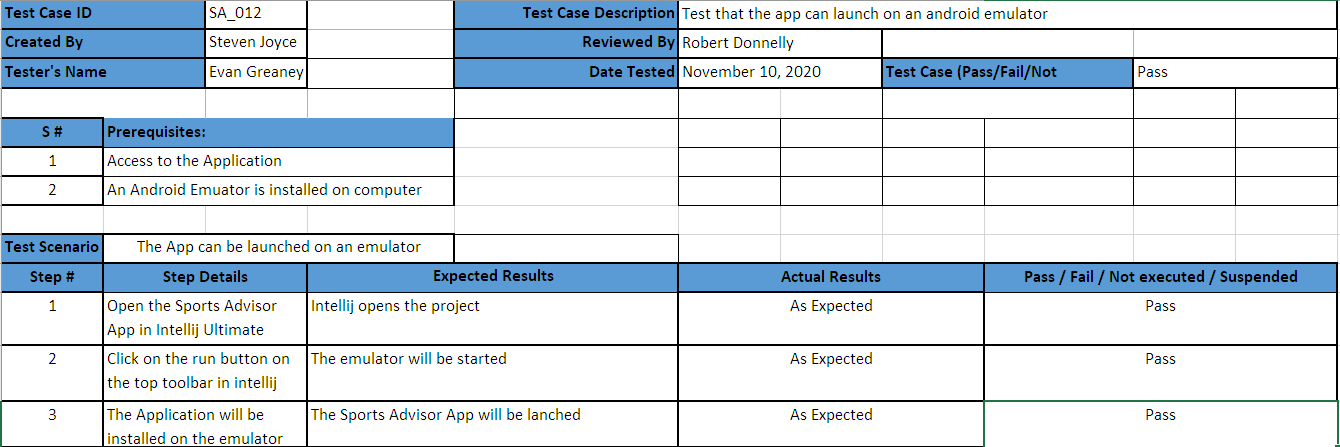
\includegraphics[width=15cm, height = 7.5cm]{img/EmulatorLaunch.PNG}
    \caption{Test Case for successful Login}
    \label{fig:altas config}
\end{figure}
The image above illustrates the test case we designed and implemented for testing the Login function of our application. The test is designed for a successful login test.
\section{Collaborative Platforms}
\subsection{Version Control}
The platform all team members were most familiar with was GitHub, it allows members to access project code versions and commit their contributions to one repository. Every team member has access to view and modifies the contents of the repository. All changes are logged and any commit can be accessed at all times, this helps with problem-solving as any issues that occur can be called back on to older commits that were functional if issues occur with the latest commit.

\subsection{Communication Tools}
\subsubsection{Microsoft Teams}
Microsoft Teams was used primarily to communicate with our supervisor. We chose this as it is linked to our student accounts and our supervisor requested us to use it as a way to communicate with them.
\newline 
Microsoft Teams is a good platform for video calls as it can be accessed on multiple platforms such as an Internet browser, Mobile/Desktop Application. It al- lows users to share files and can sync to your google drive account(file hosting service).and use a calendar feature allowing users to organize meetings.
\newline
However it is not strongly suited for messaging as its forum feature can become cluttered and tedious to navigate, This is one of the main reasons why we decided to use Discord as our primary form of communication as a team.

\subsubsection{Discord} 
Discord is a communication Application that has increased in popularity in recent years, especially considering the current pandemic. It runs on Desktop, Mobile, and browser platforms. This allowed us to always be in contact with each other if one team member's device was running into issues.
\newline
Discord allowed us to set up separate channels to sort our messages to relate to specific aspects of the Project. We could coordinate and plan different parts of the project in one place with no clutter, Each aspect of the project had a dedicated channel so that unrelated messages would not be spam our feed. For example, we had an ideas channel where we would jot down random ideas or inspiration for new features of the application, these messages would be separate from our session-planning channel which would strictly contain messages related to our sprint meetings. Due to this feature, it became our primary platform to communicate.
\newline
\subsubsection{Whats App}
We used Whats App on our mobile devices to organize our sprint meetings as a team. If for any reason a meeting needed to be held on short notice What's App was the most efficient way of coordinating a set time.
\subsection{Literature Software}
For the Development of this Dissertation we used Overleaf, we found this Latex text editor the effective way to write up due to our previous experience. The Documentation Overleaf provides is well structured which helped us with this aspect of the project. After each person wrote a part of the dissertation it was committed to GitHub, which helped with making sure every member of the team had the appropriate version of the Dissertation.

\section{Technology choices}
When choosing the technology to use in our Application, we decided to use a range of new and innovative technologies ranging from IDEs to server clients that are in different stages of development ranging from Pre-Alpha such as MongoDB Realm Kotlin Integration to Stable development with the Kotlin Language.
\subsection{Kotlin}
As a team, we wanted to learn a new programming language as a challenge for our project and to increase our skill set as Software Developers. One of our lecturers during one of our online classes from this module mentioned the Kotlin language. This led us to research this language and understand what it could be used for. We saw that Kotlin was an up-and-coming language that was primarily used for mobile Applications in Android as of September 2020 with hopes of iOS support being implemented in the near future.
\subsection{IntelliJ IDEA}
At the start of the college year, we were introduced to IntelliJ in our Distributed Systems module. We soon realised that JetBrains who are the founders of IntelliJ are also the designers of the Kotlin programming language. With this information, we decided to use this as our chosen development environment.We soon realised that we had the wrong version of IntelliJ installed on our devices. We needed to have the IntelliJ IDEA Ultimate to be able to access a Mongo Database. We got this free with the GitHub Student Developer Pack. This was an issue that was unforeseen and time-consuming but easily rectified. With JetBrains owning both Kotlin and IntelliJ writing the code was seamless and allowed testing to constantly occur. IntelliJ allowed the use of an Android mobile phone emulator to run these tests.
\subsection{MongoDB}
MongoDB is a NoSQL database service that allows a user to store data from an application for future use. The data stored can be queried in searches that outputs specific results. These results can be processed by the application and read out to the user. We chose to use MongoDB as our server because of our previous experience of developing applications with it as the back-end storage.
\newline
\newline
To use a MongoDB cluster we had to create a MongoDB Realm application. This is where the user data can be read into the Kotlin application. This can also send data to the cluster through this Realm application for storage. Realm reads in a cluster that has permission to access the stored data through a partition key and clusters data to the Kotlin application.
\subsection{JustInMind}
In order to conceptualize and visualise our application's front-end layout, we had to begin with prototyping our design. While researching design tools for mobile application development, we came across a prototyping tool called JustInMind.
\newline
\newline
It is a high-level prototyping tool used to create high-quality wireframes that allow developers to visualise their product in real-time before finalizing the design of the mobile application. It assisted us in figuring out how we want the user to navigate the application.
\newline
\newline
We tried to design the app with different orientations which can be seen in Figure 3.3 which shows the prototype for the recommended days page within the application.
\newline
\newline
In Figure 3.2 it displays the simplicity of designing features within the page on the App, this image shows how designing a prototype for a drop-down menu can be easy to design and how the design feels in correlation to the design of the page.
\newline
\newline
The Image as seen in Figure 3.1 shows the design of the prototype for the login/Sign Up page for the user, it gives a simple understanding of the basic functionality required on this page within the Application.

\begin{figure}[H]
    \centering
    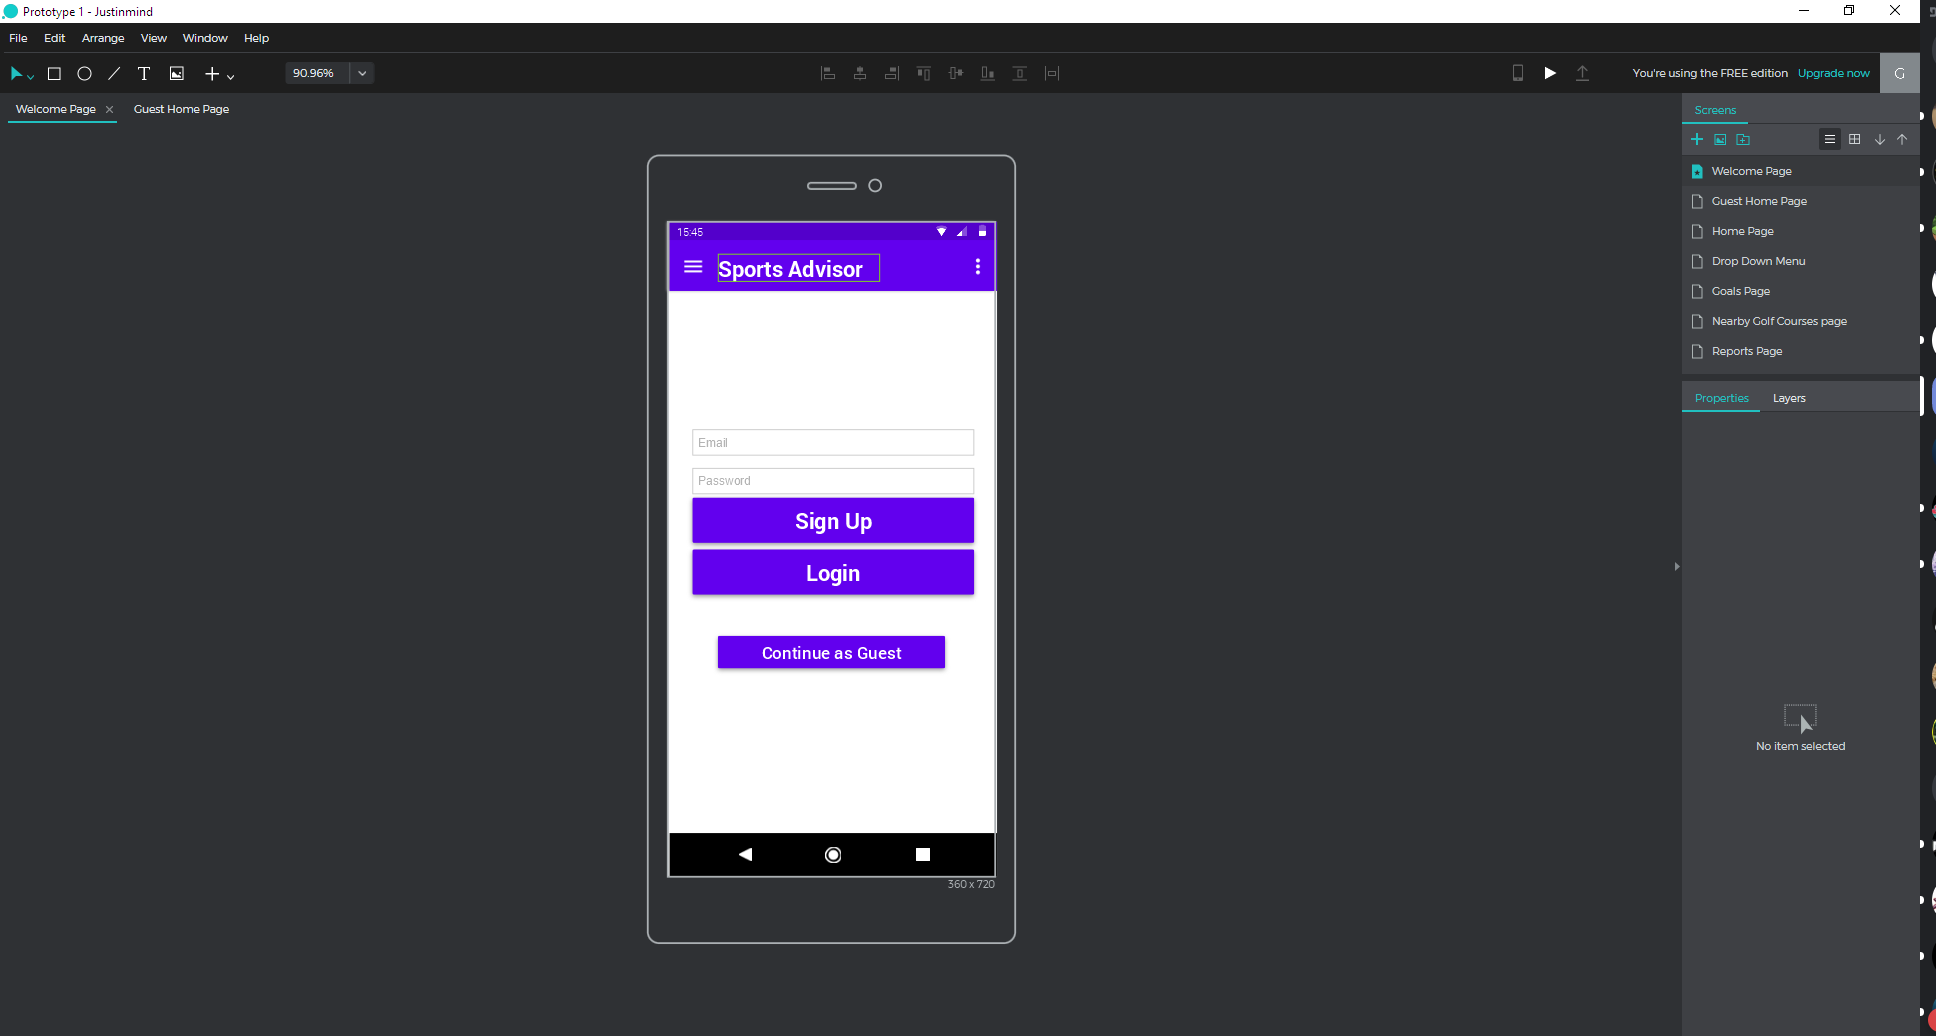
\includegraphics[width=9cm]{img/SignUpImage.PNG}
    \caption{Sign up prototype within JustInMind}
    \label{fig:altas config}
\end{figure}

\begin{figure}[H]
    \centering
    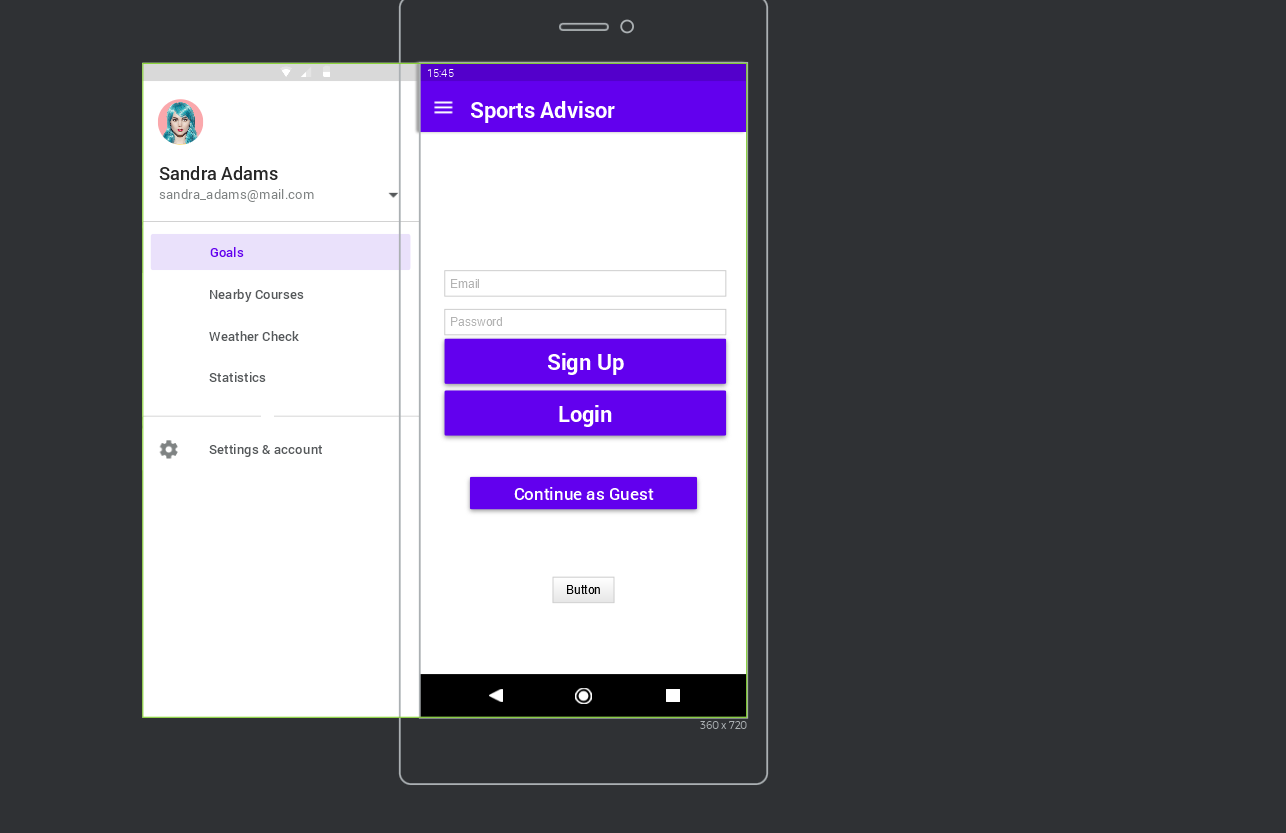
\includegraphics[width=9cm]{img/dropDownMenu.PNG}
    \caption{Drop Down Menu prototype within JustInMind}
    \label{fig:altas config}
\end{figure}

\begin{figure}[H]
    \centering
    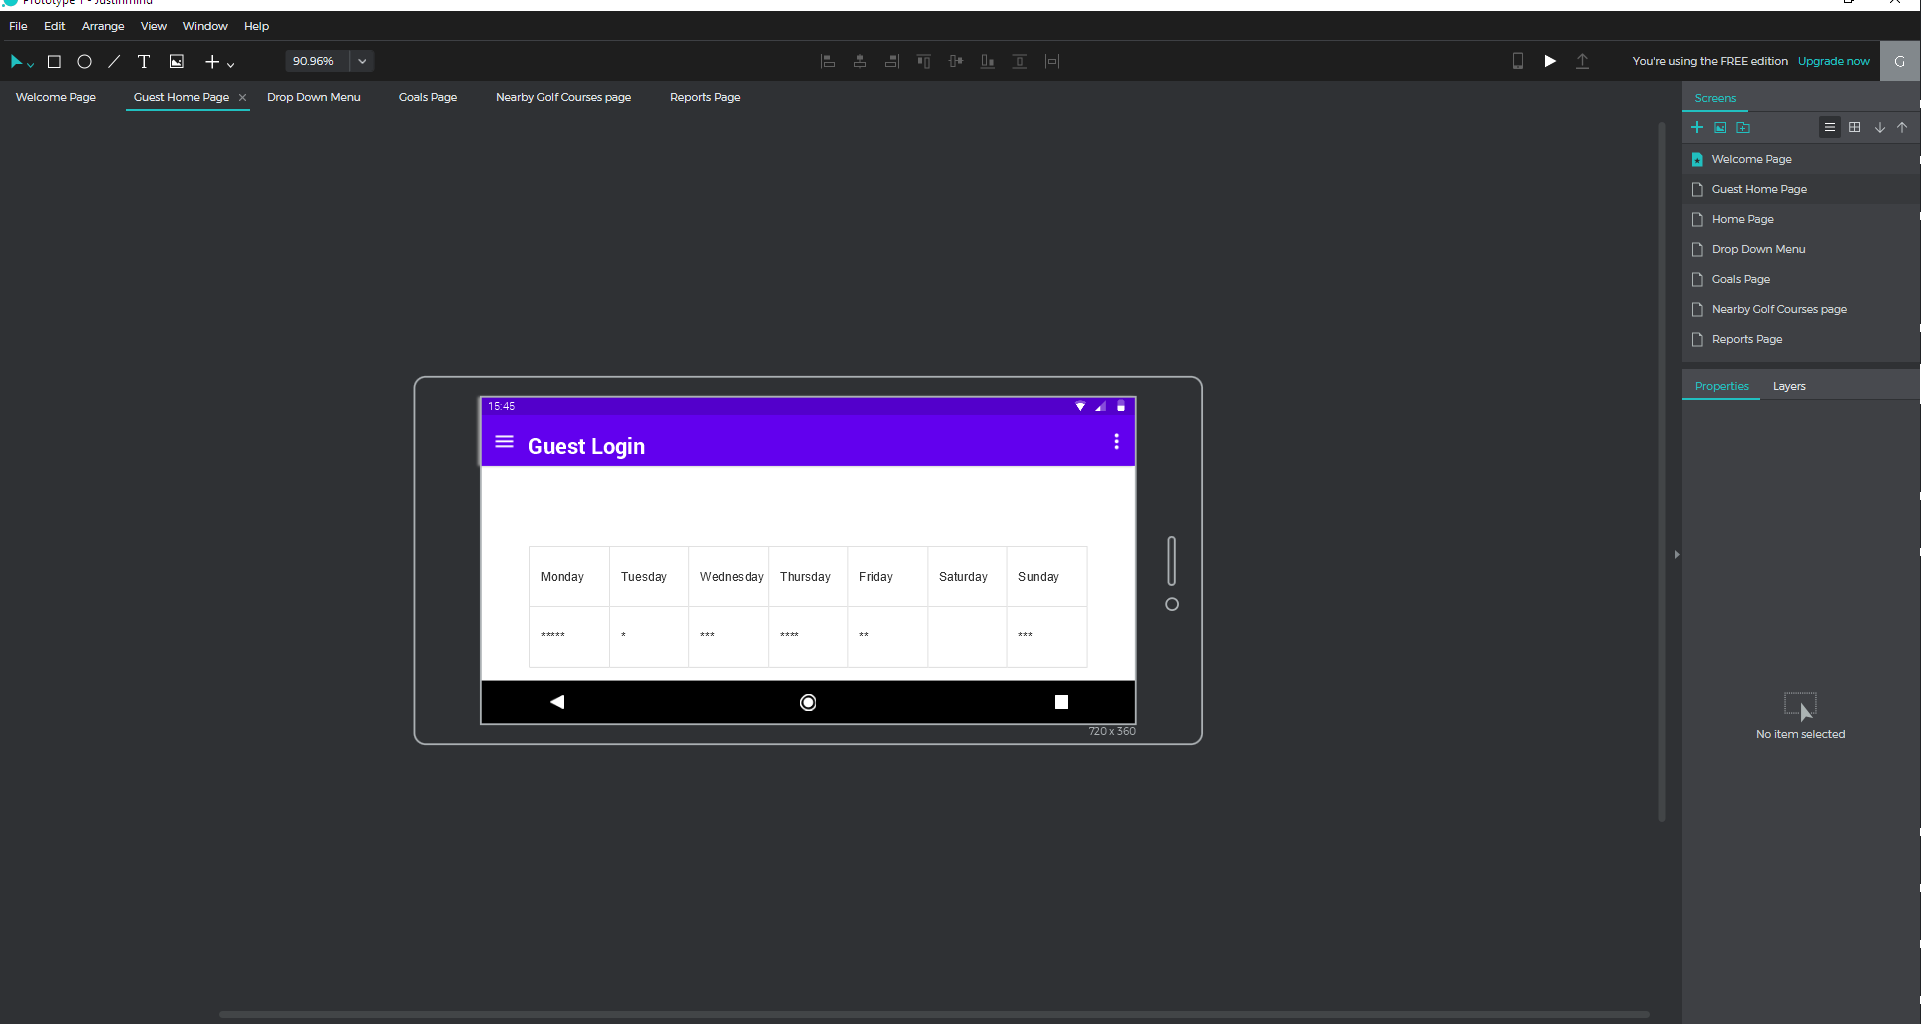
\includegraphics[width=9cm]{img/BestDays.PNG}
    \caption{Best Days to Play prototype within JustInMind}
    \label{fig:altas config}
\end{figure}

\section{Algorithm}
The algorithm we have implemented for the app is used for giving the user feedback on the weather conditions for playing golf during a specific hour on the current date. We generate JSON data from an API call and it contains an abundance of different weather variables which we have saved into variables that can be accessed in the application. We have chosen 8 variables from the list that are key to what hour is best suited to playing a round of golf. They are sunrise, sunset, hour, amount of rainfall in millimetres, temperature, wind speed, and humidity.
\begin{figure}[H]
    \centering
    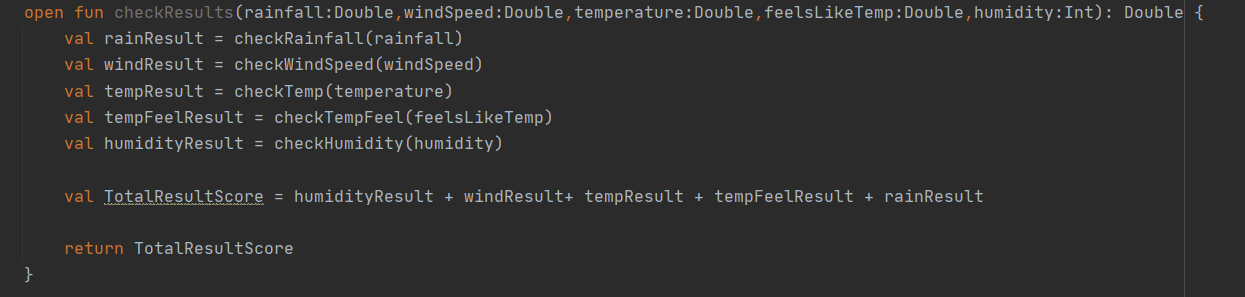
\includegraphics[width=13cm,height =6.5cm]{img/starRating.PNG}
    \caption{Star rating function}
    \label{fig:altas config}
\end{figure}
All these variables are given back to the user alongside a star rating. The star rating is out of 5, with 0 being the worst and 5 being the best. This is best understood by looking at the above image.


\begin{figure}[H]
    \centering
    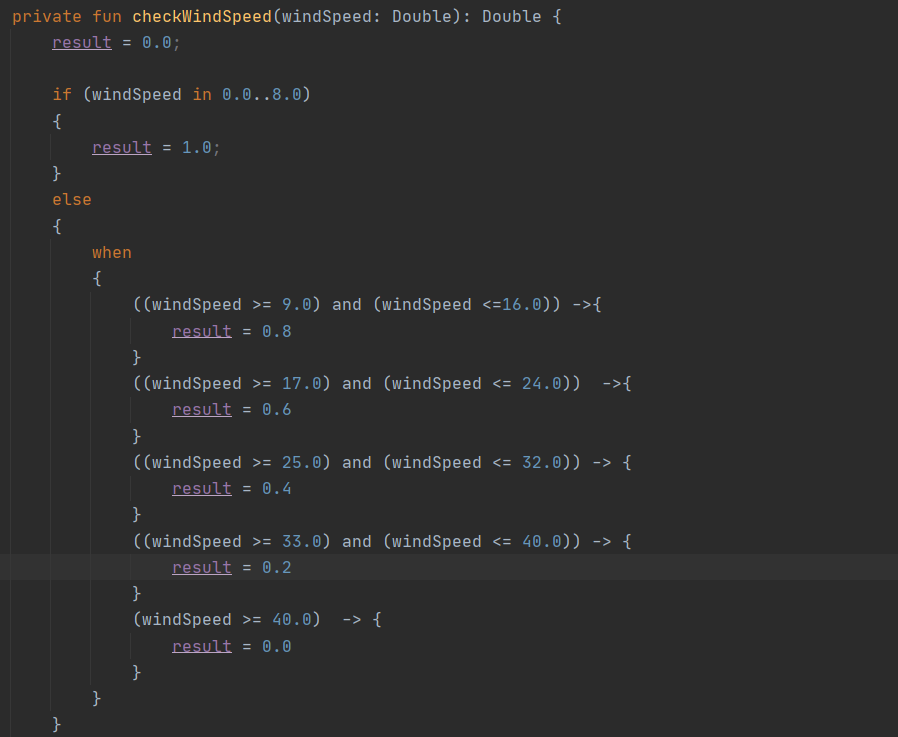
\includegraphics[width=12cm]{img/starEx.PNG}
    \caption{Wind Rating function}
    \label{fig:altas config}
\end{figure}
In the above image we illustrate how we generate a star rating for a variable, every variable is worth 1 star each but that star is broken down into a result between 0 and 1. The result is then used to generate a total score in the check Results function.
\chapter{Technology Review}
\section{Kotlin}
We found Kotlin to be less verbose, easier to read as a programming language compared to such languages as Java, C. It is a high-level language that can be used to produce mobile applications. Its coding style is similar to python but with more features and ways to implement it. \newline
This is due to Kotlin not needing any end of line syntax to allow the interpreter to move on to a new line and code being easier to understand and comprehend what the line of code is doing. - Subject to change
\newline \newline
The Kotlin language is a very good interpreter of other languages which helps when trying to write code without having a great grasp of the language. This is very important when you are beginning to learn the language or when you cannot find a way to write a method in Kotlin that you have done previously in a different language such as Java.
\newline \newline
Despite both Kotlin and Java is a native language for writing Android applications, Kotlin is seen by many as a cleaner and concise way to write code for mobile than Java. It can reduce the number of lines of code that need to be written for the application - this comparison can be seen in the code Excerpts below.
\newline
\newline
Below can be seen two examples of code one written in Kotlin and the other in Java, both pieces of code perform the same function but are equally different. As we can see in the Kotlin Code excerpt, the code tends to be more human-readable and easier to understand for people less acquainted with either of the languages.
\newline

\subsubsection{Kotlin Code Excerpt}
\begin{verbatim}
    @Throws(IOException::class)
    fun run(url: String?): String? {
        val request: Request = Request.Builder()
            .url(url.toString())
            .build()
        client.newCall(request).execute().use {
        response -> return response.body!!.string()} }
\end{verbatim}
\subsubsection{Java Code Excerpt}
\begin{verbatim}
    OkHttpClient client = new OkHttpClient();
    String run(String url) throws IOException {
        Request request = new Request.Builder()
            .url(url)
            .build();
        try (Response response = client.newCall(request).execute()){
         return response.body().string(); }}
\end{verbatim}

\subsubsection{Limitations of the Kotlin Language}
Kotlin comes with many amazing features that assist the Developer in writing efficient and easy-to-understand projects and Applications but with all of these innovative and useful tools that come with the Kotlin language, it is always changing. As the Kotlin programming language is relatively new in comparison to other programming languages such as Java and C++, the language itself and its components vary in stages within a Software release life cycle, an example of which would be the Kotlin/JVM is in stable development since version 1.0 but the component for Multiplatform projects is in Alpha version 1.3 as of the 11th February 2021 which can be seen in Figure 4.1.
\begin{figure}[H]
    \centering
    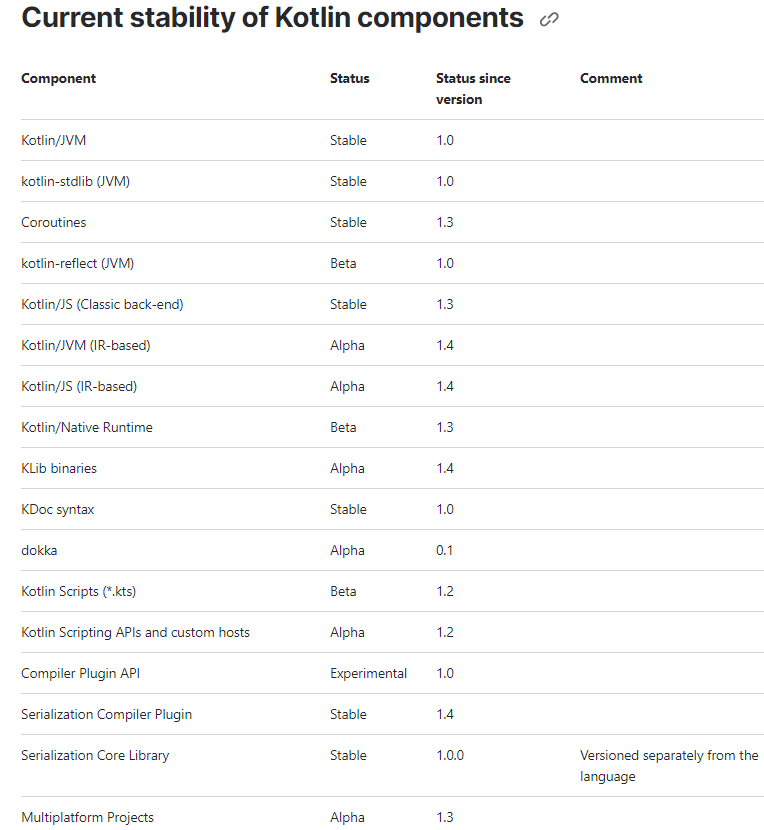
\includegraphics[width=11cm,height = 11cm]{img/KotlinStability.PNG}
    \caption{Stability of Kotlin and its components}
    \label{fig:altas config}
\end{figure}
Due to the Multiplatform component not being in a stable release version, we decided to solely focus on development for Android devices as this is included with the stable release of Kotlin/JVM and along with our experience in creating applications for Android devices during our time at GMIT.
\newline
\newline
We initially created our base Application with the intention of utilising the multiplatform component for our application. We soon found that it was very difficult to run and in some instances would not compile and would some- times render the Application completely inoperable. This came as a cause for concern for us in the early stages of development and initially delayed our development by two weeks. It made us reflect on the feasibility of the component and if it would cause major issues later on in the development life cycle of the Application and as a result was ultimately removed from the Application due to being too unstable, with a new project entirely designed for the Android platform being created instead.

\section{IntelliJ IDEA's}
The development environment provided by IntelliJ allows for the development of several different types of programs including Mobile Applications. The IDE contains a built-in android development environment with Kotlin being the default language.
\newline
\begin{figure}[H]
    \centering
    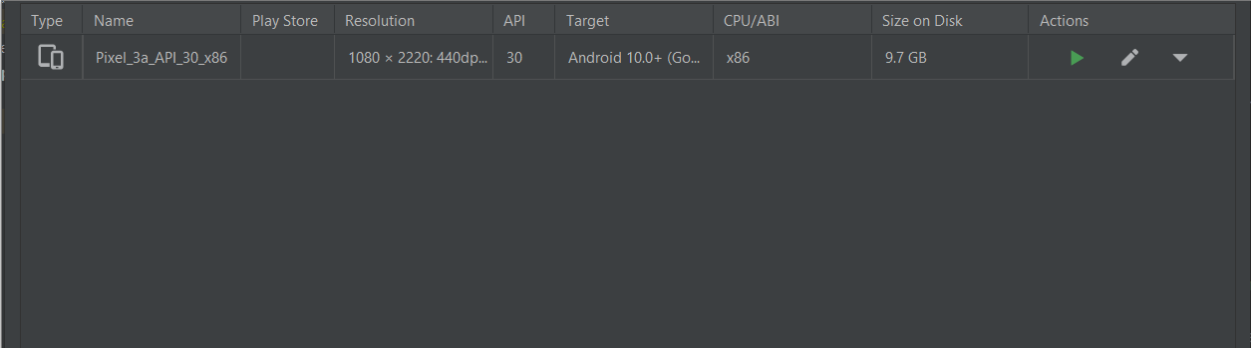
\includegraphics[width=15cm]{img/androidADK.PNG}
    \caption{Android Device Kit}
    \label{fig:adk menu}
\end{figure}
The image above shows the emulated device customisation menu. In here you can add a virtual device to run the android application on. The ability to modify what Android SDK used within the IDE was very important for testing the project. That feature is a great way to debug a mobile application efficiently and in real-time.
\begin{figure}[H]
    \centering
    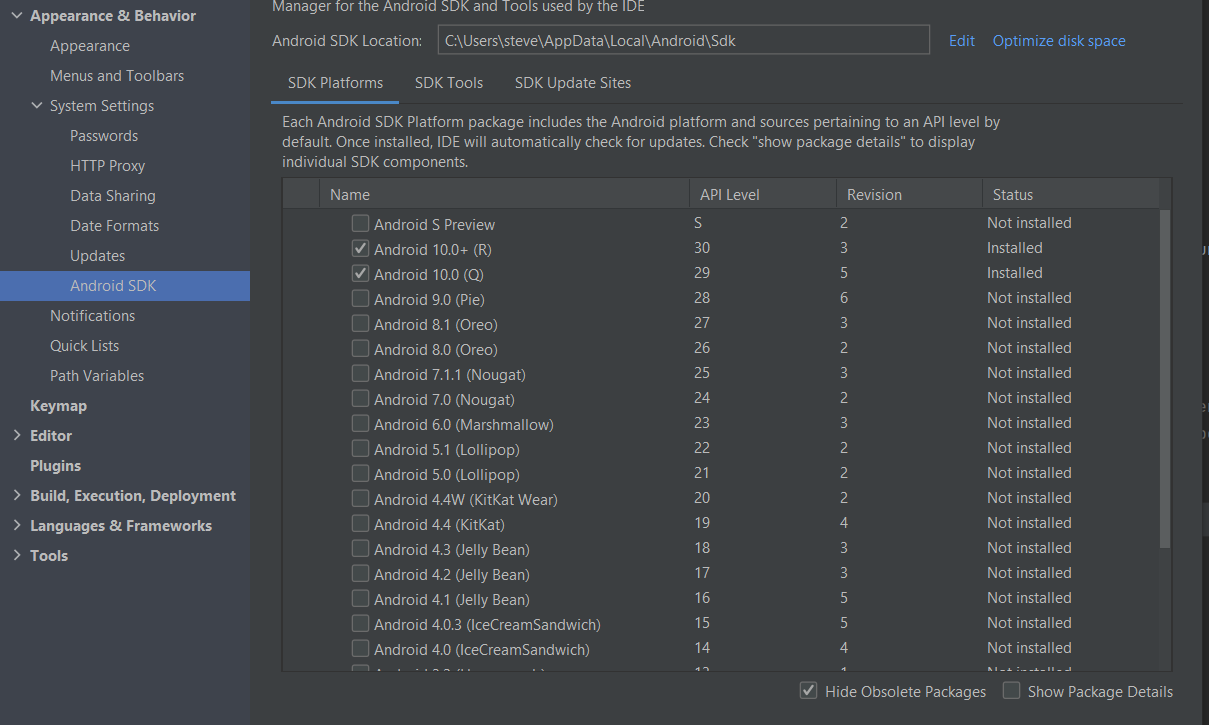
\includegraphics[width=12cm]{img/androidSDK.PNG}
    \caption{Android Software Development Kit}
    \label{fig:sdk menu}
\end{figure}
The SDK manager on IntelliJ allowed us as developers to run the application on different versions of the Android system. When you choose an SDK, it gives you a percentage of how many people who use Android will be able to use your device. The more up-to-date version - meant fewer people could run the app, we when with the Android Oreo version for our virtual phone which is Android 10.0 but we set our minimum SDK version to 28. This allowed the phone to run on Android 9.0(Pie) as well as the version we set up on the virtual device.
\section{API's used}

\subsection{Open Weather API}
Open Weather is an API that allows the user to retrieve weather data from any location using its NWP (Numerical Weather Prediction) Model. This API has been designed to be used universally in any Language to gather data. It gathers this data using a proprietary convolutional neural network that collects and processes a wide range of data sources to cover any location and
consider the local nuances of climate.
(Quote from https://openweathermap.org/guide - Openweather NWP model)

\subsection{Geocoding API}
In order to retrieve data with the Open Weather API, we needed the longitude and latitude of a chosen golf course selected by the user. With the help of the Geocoding API, it gives the ability to convert street name data into longitude and latitude values for the Open Weather API to search weather data based on that location.

\subsection{AccuWeather API}
After a lot of testing and attempting to retrieve data using the Open Weather API and Geocoding API, we found it was very difficult to retrieve, store and convert the data from XML that was provided by the Open Weather API, we then came across the Accuweather API that searches for locations based off of their own location codes which we then use to offer the user a list of golf course locations within Co. Galway that they could choose from instead of having to search for courses themselves.
\newline
\newline
By offering this list we can accurately show the conditions for these particular golf courses of choice instead of being able to search for weather conditions for cities and towns instead of the actual golf courses.
\newline
\newline
The data provided from the API is then able to be processed by our Algorithm to provide a rating for the conditions based on two search features, a 12-hour search for that particular day or a search based on the next 5 rolling days, the 12-hour search will provide the rating based on the next twelve hours and will provide a rating for those hours, and then the current conditions search will give a general rating for the current hour when accessed by the guest functionality.

\section{MongoDB}
To utilise the MongoDB database, we had to use two of its three main core features. The two features we use were Atlas and Realm, Atlas and Realm can be integrated in a way that allows for a seamless connection to and from the Android Application. The MongoDB Atlas uses a server that can be either free or paid for use by a set charge per hour. We choose a free tier server based in N.Virginia (us-east-1) run by Amazon Web Service(AWS). This server was chosen because the Irish server does not work with MongoDB Realm as the server for Ireland is only using MongoDB version is 4.2 but Realm runs on MongoDB version 4.4 and above.
\subsection{Cluster}
It is the word associated with having several MongoDB servers working together. MongoDB distributes data in 2 ways: replica set and sharded clusters. The main objectives of a MongoDB cluster are to be able to read and write several nodes. The data is separated into the different nodes of the fragment.
\begin{enumerate}
    \item \textbf{Replica Set:}
    \newline This is when the data is sent across several servers without the data changing. This is a layer of protection from a server failure.
    \item \textbf{Sharded Cluster:}
    \newline  This is where the data is fragmented into parts of the data to be carried by a different server. This is done to have larger datasets and have better performance.
\end{enumerate}
\subsection{Atlas}
Atlas is the area in which data is stored within the MongoDB system. it allows its users to create a database for a specific user that will only store their data in a collection. \newline
This is great for protecting user data. The data can only be accessed by inputting a user id. This user id is unique and is also the user’s username that will be always shown in the application. It is the 1st thing a new user will input in the application when creating an account. With the data for a user protected in a cluster, this allows the application to output data to the user that is only relevant to them. That feature was a major reason for using MongoDB in our application.
\newline
The user can store the name of the golf course they played at and the score they got that day. It will also save the par for the course that date and the overall total score for the round of golf.

\begin{figure}[H]
    \centering
    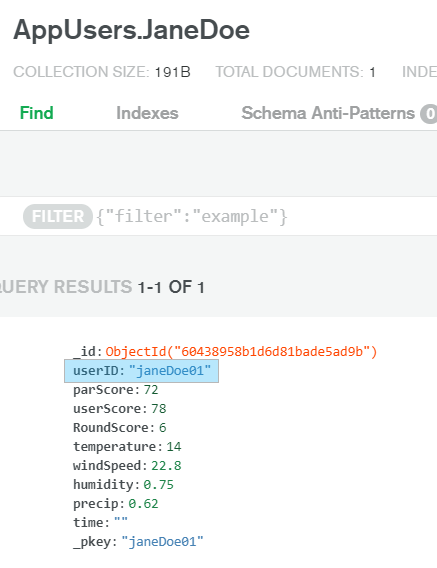
\includegraphics[width=9cm]{img/UserDatabase.png}
    \caption{MongoDB database with a User}
    \label{fig:altas config}
\end{figure}
The highlighted field in the above figure is the authentication key that will need to be inputted by the user to access the database associated with them. Without this key being correctly inputted, the user will not get any data from the MongoDB cluster. This is how MongoDB protects user data.
\subsection{Realm}
The Realm feature of MongoDB is how MongoDB now interprets a Mobile Application. It creates an application that can be used to access a cluster - The cluster is what Atlas creates to store the user data.
\newline
The App will have a unique ID that is called in the Mobile Application back-end to link your application to MongoDB. It creates a user that is linked to a specific database in the cluster. This user can only be authenticated by entering the correct email and password. The app can and does have rules that limit what data a user can access to modify or view.
\begin{figure}[H]
    \centering
    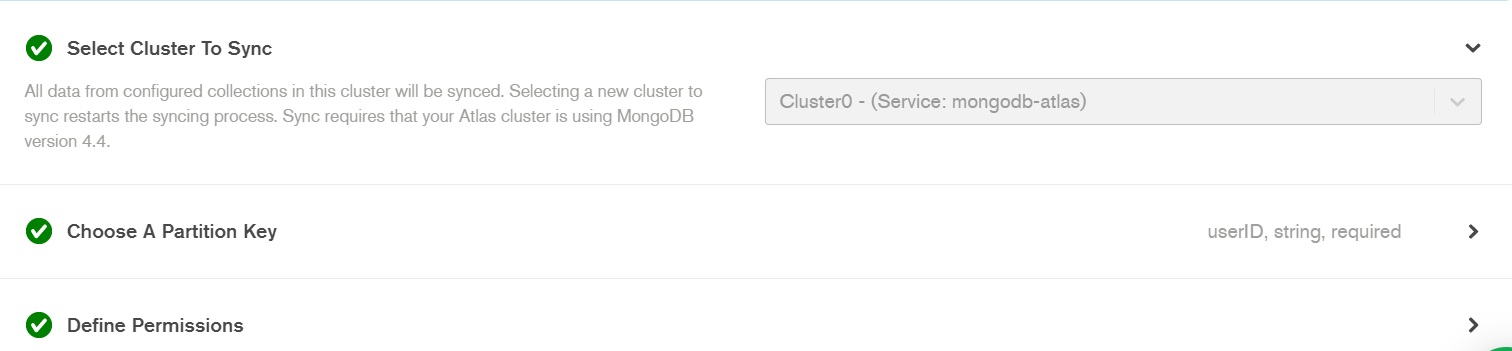
\includegraphics[width=15cm]{img/syncSetup.PNG}
    \caption{MongoDB Sync configuration}
    \label{fig:altas config}
\end{figure}
The above figure is an image of the MongoDB sync configuration. This is where the developer connects to the Atlas cluster by implementing a partition key. This key is how a cluster is made available to the user. The permissions for what a user can do with the database it has connected to are set here as well. We have allowed the user to both read and write to the collection but the data is protected by the userID key created in the collection itself.\newline
For this project, Realm functioned as the middle man between the application and the MongoDB Server. It allowed the data to be sorted in a manner in which is easy to understand and utilize. Despite the Realm Sync still being in a developmental phase, it is of a high enough standard to work with no issues on their end. \newline
We have been contacted by the MongoDB Realm to give feedback to help them see what issues have occurred and if it has worked well for us.
Realm allows the creation of App users. This is the best way we found to make data private and protected. The user will have to log into the server with their username, email, and password. These are created in the app and are stored on the Realm App external storage system.

\begin{figure}[H]
    \centering
    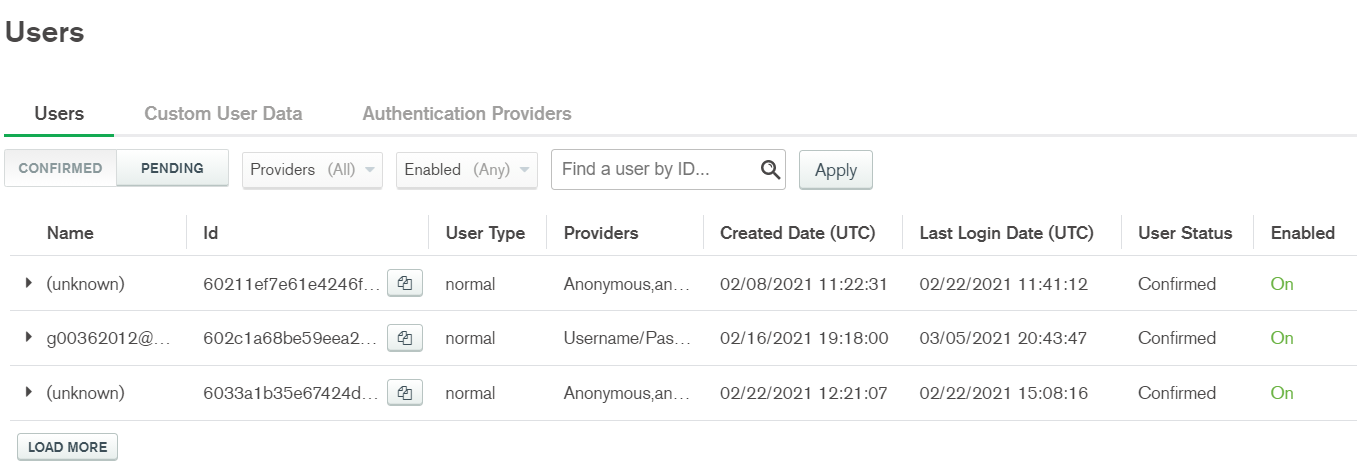
\includegraphics[width=15cm,height = 8cm]{img/Users.PNG}
    \caption{MongoDB database with a User}
    \label{fig:altas config}
\end{figure}
The image shown above in figure 4.3 is a snippet of the User database on the Realm App. The realm app will create a temp user for a guest to get a quick API call that shows the weather outlook for the next 24 hours. The multi-day weather report is only available for users who have logged in. The user needs to log in with an email and password.

\section{GitHub}
GitHub is the code hosting platform we used for our project which allows us to track and manage our source code with version control in a collaborative fashion. We used a private repository which allowed us to control who could access our code as well as who could contribute to our code. It allowed us to use branches to merge our code so we can work on separate features and not worry about breaking each other's code. \newpage
Since it is directly connected to git, we were able to push and pull code directly from the terminal which we had experience in, and as a result, was our preference over using IntelliJ's inbuilt GitHub features. The GitHub website has a solid user interface, the service is stable and reliable so we had no worries about hosting our code on their site. GitHub also offers a student pack which gives students free access to developer tools that we incorporated into our project including Mongo Realm and IntelliJ Ultimate.
\section{Communication Application's}
\subsection{Discord}
Discord is a free instant messaging and Voice over Internet Protocol service which is generally targeted for gaming or other online communities to communicate together on servers. Our group was already well acquainted with its features and was comfortable with setting up our own server for the group's project. Discord is very similar if not identical to the untrained eye to the business communication platform Slack which is used by businesses in a workplace environment the main difference being that Discord is completely free whereas Companies pay a fee to use Slack. Discord then served as an appropriate alternative to Slack as it offered the same features including persistent chat rooms organized by topic, private groups, direct messaging, screen sharing, and online voice meeting capabilities.
\newline
\newline
We found
\subsection{Teams}
Microsoft Teams is a collaborative workspace that is fully integrated with Microsoft Office 365 Services, Teams allows for scheduled voice and screen sharing meetings to be arranged via a calendar layout so that users can organise multiple meetings throughout a day to as well as schedule meetings to automatically occur on a daily, weekly or monthly basis such as in our case we were able to set up our meeting with our supervisor to automatically schedule itself each Monday at 11:30.
\newline
\newline
We also found Teams to be a lot more user-friendly to users who are not as technologically skilled, rarely does Teams encounter voice chat or microphone connectivity issues. It has both a desktop application and a browser application formats for users on computers which allows flexibility for a user who might be borrowing a machine or have low storage they can use the web app version through a browser.
\newline
\newline
Similarly, users can use an android or ios app for when the situation is more suitable for example replying to a direct message or meeting invitation whilst away from their desktop or laptop device. Its also worth noting that if a team is using an Office platform such as Excel, PowerPoint, or Word, the members of the team can work on the same document at the same time which is a major advantage for people using Office platform tools. The only downside of teams which is a common criticism of Microsoft software would be its UX can be frustrating, while it has improved in recent updates the UX is nowhere near as smooth as Slack or Discords in terms of navigating teams or groups you are a part of and its message feeds.

\section{Dissertation Proof-Reading Tools}
When we began writing up this document, we wanted to use a tool to check the grammar used, give a guide to what changes need to be made and overall make this document more easier to read. We realised this when we started to give our supervisor the document to get constructive feedback on what we can improve on.  To combat this we decided to use Grammarly. \newline \newline
Grammar is one of the most popular tools used for proof reading documents.  It allows the user to upload a file of any size and get it read within a minute of uploading the documents. The only issue we had with this tool is that it would give hints to change the way words are written into the American variations of English words such as \"colour\" or \"realised\". It wanted us to change those 2 words into \"color\" and \"realized\". The hints it gave helped us convert sentences into words that better convey what we wanted to say.
\newline \newline
With the use of Grammarly we were able to fix any grammatical errors of the document within half an hour and without having to read the document repeatedly. It allowed us to work efficiently and manage our time better. Grammarly is able to be added to a browser with an extension or as a desktop app on windows. The ability to use it in many locations on a computer device made the use of it more convenient. \newline
Here is a link to the Grammarly website: {\url{https://app.grammarly.com}}
\chapter{System Design}
With our system, we have three main layers that integrate with one another to build our functional application. The Front End part of the application deals with the visuals and functionality that will be delivered to the user. It communicates with the Back End of the application which stores and retrieves data for the user upon interacting with the front end’s elements. The Data Retrieval tools are used in collaboration with the Front End to retrieve and present the current weather data for now and the next twelve hours as a set of ratings for the optimal playing conditions for each hour.

\section{Front End}
\subsection{Android}
\subsubsection{Navigation}
\subsubsection{XML}
\subsubsection{Activities}
\subsubsection{Fragments}
\subsection{Kotlin}
\subsubsection{classes}
\subsubsection{Algorithm}
\subsection{Gradle}
The Gradle is a build system used for building an application. For Android, it is used to build, test and deploy the application to an Android device.
\newline \newline
With Android, a Gradle folder is essential, due to it being used to generate an apk from the kt and XML files that have been written in the project. The Gradle folder looks through all the files in the project and converts them into dex files before putting all the data into a single file that is in an apk format.
\newline \newline
The Gradle folder is located in the root directory. This folder contains all the dex and apk files that run the application. The project contains 2 build.gradle, one located in the root directory, and the other is located inside the app folder. The root file applies what version of Kotlin the application is written in and all the dependencies of the application such as MongoDB Realm. \newline \newline
The file set in the app folder applies the android version associated with this application and all the dependencies that are needed to utilize that version of Android in this app. The ability to sync the application with MongoDB Realm is set to true here, this allows the app to read, write, update and delete collections stored in the MongoDB database.

\section{Backend}
With our application, we set up a MongoDB server to allow a user the ability to create an account to store their golf course results. To allow the user to access the MongoDB server we needed a register user page and a login page.
\subsection{MongoDB}
\subsubsection{Realm}
To connect to MongoDB, the application uses MongoDB Realm. This is an application on the server-side which allows the android application to access the MongoDB Atlas Cluster. The ability to access this only occurs for users who have registered. The email, password, and userID act as a way to verify who is trying to connect to the data while also filter what data can be seen on the User History page.
\subsubsection{Atlas}
The MongoDB Atlas is where the MongoDB database is located. A MongoDB Atlas cluster consists of a collection and a database. To connect to this database.
\subsection{Integration}
\subsubsection{How the user can register for MongoDB Cluster Access}
\begin{figure}[H]
    \centering
    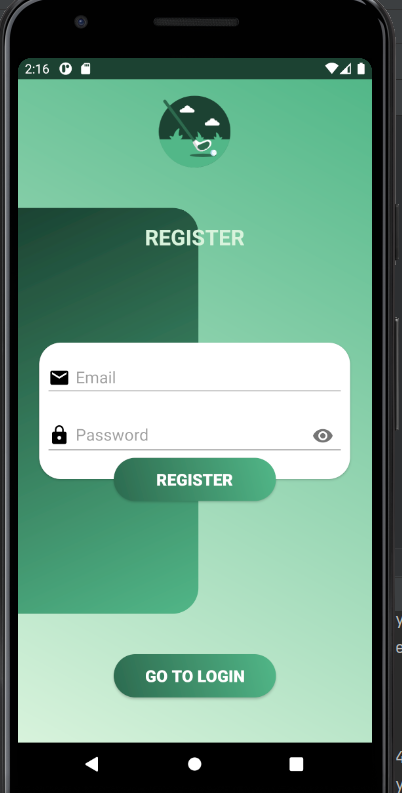
\includegraphics[width=7cm, height = 13cm]{img/registerPage.PNG}
    \caption{Page for registering a new user}
    \label{fig:altas config}
\end{figure}
The above image is a screenshot of both the login page that is used to register a new user for MongoDB server access. To create a user the person who has opened the application needs to input an email and a password. If the user input has not been accepted the user gets an alert. That alert info will be different depending on what input error has occurred. If the user input is accepted an alert comes up saying: User has now registered - now click GO TO LOGIN.
\begin{figure}[H]
    \centering
    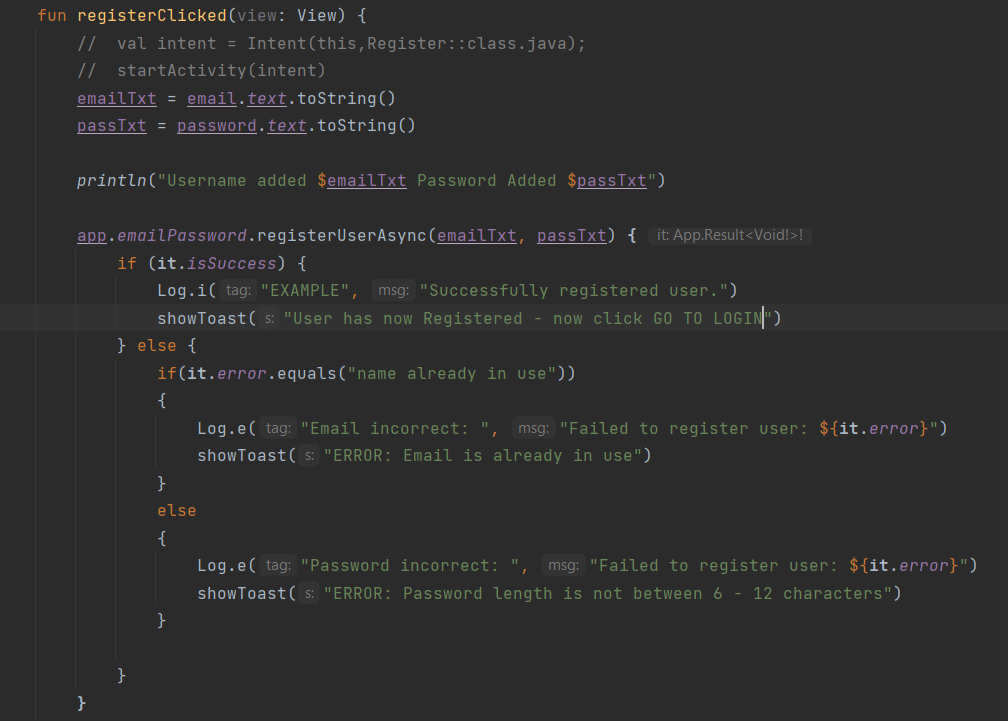
\includegraphics[width=11cm, height= 8cm]{img/registerCode.PNG}
    \caption{Code associated with the register page}
    \label{fig:altas config}
\end{figure}
Above is an image that depicts the code that is used to register a new user for MongoDB server access. To create a user the person who has opened the application needs to input an email and a password. If the user input has not been accepted the user gets an alert. That alert info will be different depending on what input error has occurred. If the user input is accepted an alert comes up saying: User has now registered - now click GO TO LOGIN. The GO TO LOGIN button brings the user to the login page to sign into the MongoDB server to access the user data that is attached to that user. 
\newline
The user input fields are saved as emailTxt and passTxt string variables by utilizing the toString function in Kotlin. The string variables are passed into the function app.emailPassword.registerUserAsync() to be sent to the MongoDb Realm to create a new App user.
\subsubsection{How the user can login to the MongoDB Cluster}
\begin{figure}[H]
    \centering
    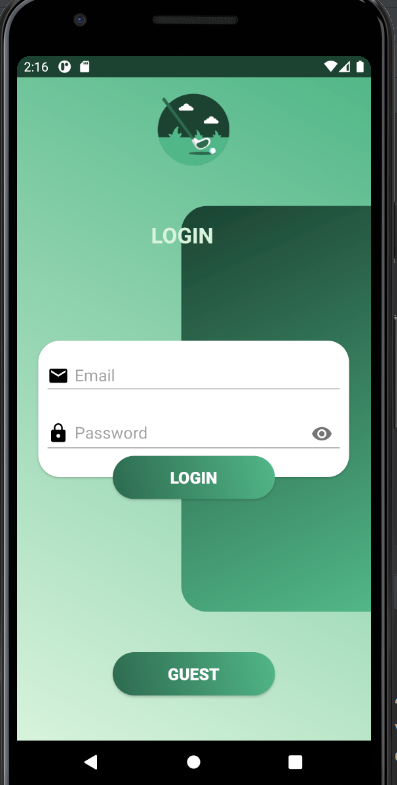
\includegraphics[width=7cm, height = 14cm]{img/loginPage.PNG}
    \caption{Page for logging in a user}
    \label{fig:altas config}
\end{figure}
To connect to the MongoDB server, the user needs to input their login details into the application when they are on the Login Page. The page can be seen in Figure 5.3 to the MongoDb Realm Application. When the user is on the login page it will enter its userID, email, and password again. The user will get an alert saying successfully logged in UserID.

\begin{figure}[H]
    \centering
    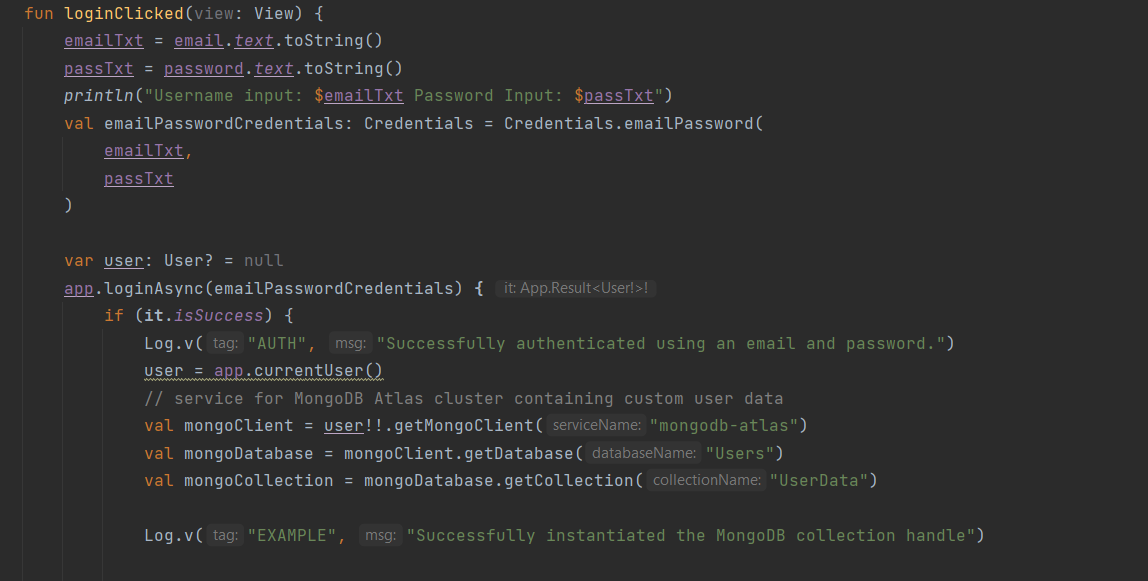
\includegraphics[width=11cm, height = 11cm]{img/mongoSignIn.PNG}
    \caption{Code associated with the login Page}
    \label{fig:altas config}
\end{figure}
By using the MongoDB loginAsync method for signing into the server we can get back an error if the sign-in was not successful and this method also allows the user to read and write to and from the database.
\newline
The application also gets back the data the user has stored up in the server. It finds the data by searching the database for a unique identifier. That unique identifier is the userID. The userID is the partition key for the MongoDB Atlas database, This allows the MongoDB database to be filtered for use in the user history page. The output is only the data that the current user of the application has sent to the MongoDB server. \newline
If the user has not saved any data an alert will appear on the device with \" a No User history Found \" outputted. The use of alerts may be minor but it has a big effect on the user experience. The ability to know what error you have when trying to run a specific function is key to solving that issue, this is where the use of alerts in the application is very effective.
\newpage
With our application, we also send data to the server. That data is generated on the score page. The score page lets the user store results from a full round of golf including the course par score and user round score. The nett score for the round of golf is generated by taking the handicap away from the user’s total round score.
\begin{figure}[H]
    \centering
    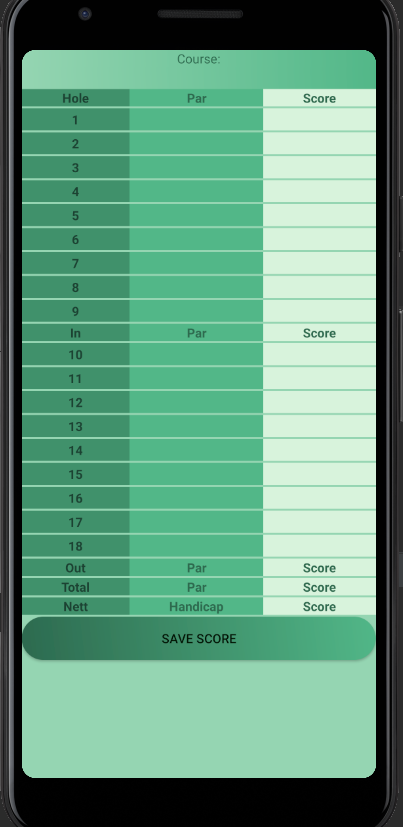
\includegraphics[width=7cm, height = 13cm]{img/scorePage.PNG}
    \caption{A snippet of the score page}
    \label{fig:altas config}
\end{figure}
When the user presses the save data button, the round is saved in the application before that saved data is sent to the MongoDB database to be stored in a collection.
\newpage
The image below illustrated how we are sending the data collected on this page to the server. It is done by calling the send data function.
\begin{figure}[H]
    \centering
    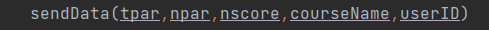
\includegraphics[width=11cm]{img/sendDataFCall.PNG}
    \caption{Calling the function for sending the data to the server}
    \label{fig:altas config}
\end{figure}
The values sent to the function are all processed on the score page. tpar is the course par score, npar is the course handicap the user has assigned for that round, nscore is the users total score for the round when taking into consideration the handicap. The courseName is the name of the course the user is playing at and the userUD is the unique username that the user has created for itself.
\begin{figure}[H]
    \centering
    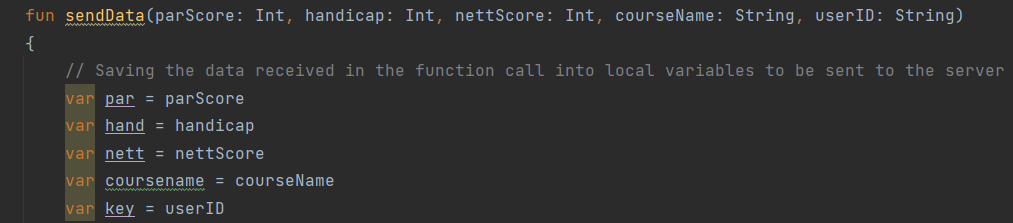
\includegraphics[width=11cm, height = 2.5cm]{img/sendDataFunction.PNG}
    \caption{The function used sending the data to the server}
    \label{fig:altas config}
\end{figure}
The image above shows how the function stores the data it receives from the function call to be used in the code shown below. We receive the data collected on the score page and save it in local variables that are used to send that data to the MongoDB server in the method illustrated below.
\begin{figure}[H]
    \centering
    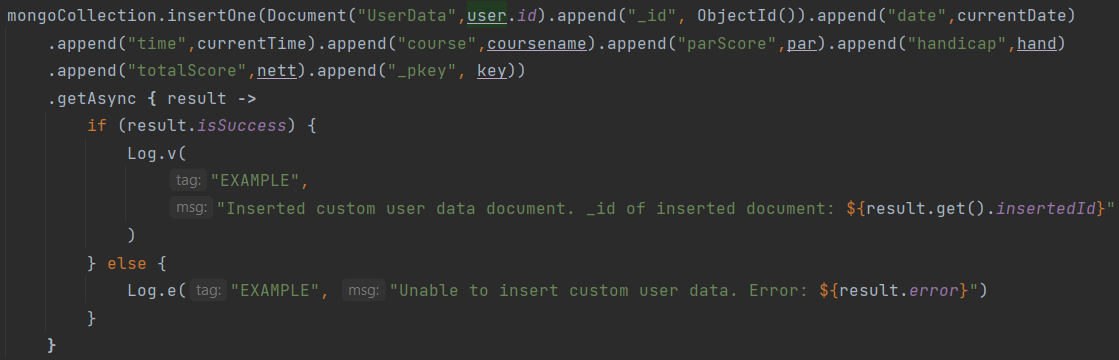
\includegraphics[width=15cm, height = 6.75cm]{img/sendServer.PNG}
    \caption{How the data is sent to the server}
    \label{fig:altas config}
\end{figure}
With MongoDB Realm, there are several different methods built into the system that can be used to perform CRUD operations. Crud operations stand for Create Read Update and Delete. These are the staples of any MySql or NoSql service. Without them, they would be useless. The function insertOne allows a user who has credentials to send the data to the server.
\newline
The collection has a name that needs to be called to start the process, our collection is called UserData. The use of append allows the creation of new values to be stored in fields already associated with the collection. The fields we have set up are id, date, time, course, parScore, handicap, totalScore, and userID. The data we send up to the server are the values received in the function call. Those values along with the current date and time. The date format is DD-MM-YYYY while the time format is Hours-Minutes-Seconds. Those 2 values are generated when the function is called for the exact date and time. They utilize the java SimpleDateFormat Class to generate the time and date in the format that we wanted and while giving back the correct results.
\subsubsection{How the data received is outputted to the User}
\begin{figure}[H]
    \centering
    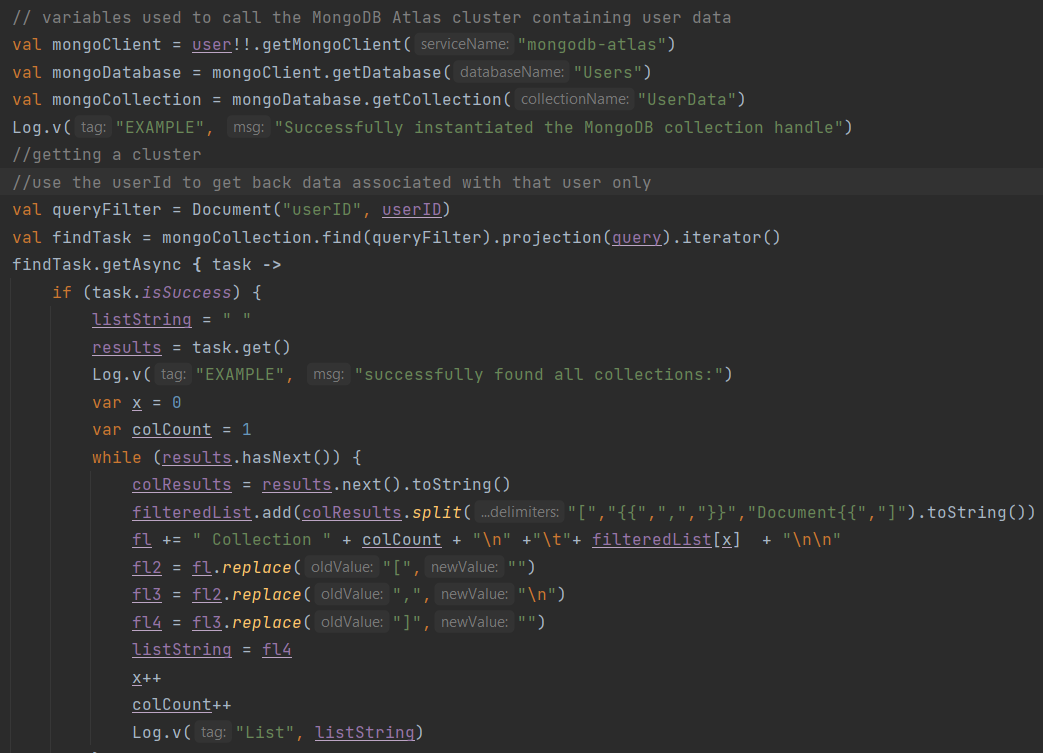
\includegraphics[width=15cm, height = 9cm]{img/getMongoDBdata.PNG}
    \caption{Code snippet of how the data is sent to the server}
    \label{fig:altas config}
\end{figure}

\begin{figure}[H]
    \centering
    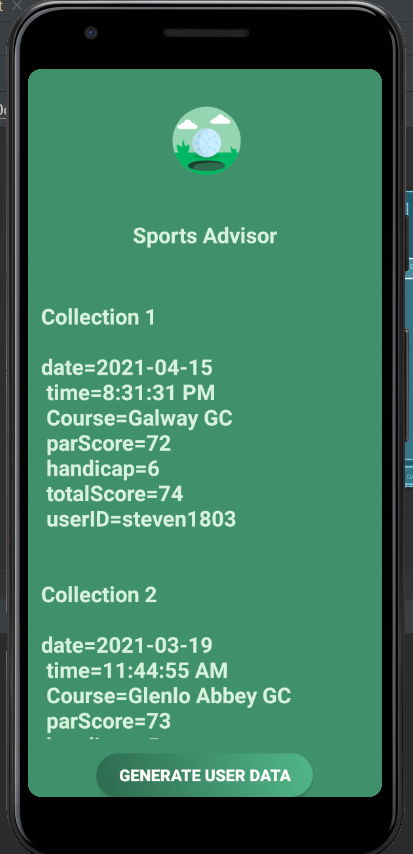
\includegraphics[width=6.5cm, height =12cm]{img/userHistoryPage.PNG}
    \caption{How the data is sent to the server}
    \label{fig:altas config}
\end{figure}

The data is received and shown on the User History Page. When the page is opened the MongoDB collection is called and the collection data is saved in a string. This string is then outputted to the app when the Generate User Data Button is pressed. \newline
The page has an onCreate function that contains the code in Figure 5.9. The code allows the MongoDB database to be filtered by the userID to output only the data that is associated with that id key. The userID is set on the settings page. This is how we protect the user's data and stop unauthorized access to data stored on the database. All userId values are unique. The data is outputted in order of oldest stored data to the latest stored data. The outputted data is the date, time, Course, parScore, handicap, totalScore, and userID with a line separated between each output for better readability.

\section{Data Gathering and Processing}
For our application, one of the major parts of the project was to retrieve weather data from a weather API using the OKHTTP: HTTP and HTTP2 client. This data is then gathered and then parsed from Strings and Objects to their JSON representations using GSON. This data is then processed and after reading in all the data, a rating between 1 and 5 is then applied to an hour associated with the weather values passed in.

\subsubsection{AccuWeather}
One of the main aspects is retrieving data from the AccuWeather API, this was fundamental part of the app as without it, hourly ratings based on conditions for playing golf couldnt be shown to the user for their chosen golf course. We decided upon implementing Accuweather as part of our Application as it was able to search for locations based on their own specific location codes, which then allowed us to create specific locations of golf courses in Co. Galway on a list for the user to pick from.

\subsubsection{OKHTTP}
For our data retrieval we used Okhttp to gather the weather data from the Accuweather API,we decided upon this as the technology to retrieving data because of one its main features, its perseverance in poor network conditions or when the network is being troublesome: "it will silently recover from common connection problems. If your service has multiple IP addresses, OkHttp will attempt alternate addresses if the first connect fails."\cite{ref1}
\newline
\newline
This is vitally important to the design of our Application as we know that not every golf course will have good WiFi at their clubs and then when the player is on the golf course they may have to use their mobile data and in certain locations, the mobile data may be poor or non-existent so by using this technology, it will still try to make these requests even under the poorest of conditions.

\subsection{GSON}
After OKHTTP retrieves the data back from the Accuweather API service it returns back string values and objects that need to be parsed into JSON Representations of that data so that it can be processed into ratings, this is where GSON comes into play, it takes the data and converts it to JSON readable data, this is then stored into multiple Kotlin data class Files which can then be called upon to calculate the ratings for the hour.

\subsection {Processing the Data}
When the data has converted from a String to its JSON Representation, it is then time to take that data and compare it to predetermined values which will check to see if data that is being passed through fits inside any of of the ranges of values it will be given a value between 0 and 1.
\newline
\newline
There are six different types of data that are passed through to the data processor, these include Rainfall, windSpeed, temperature, real Feel temperature, Humidity, and if the hour is in daylight. The first five values determine the rating out of 5 and each one of these values are rated between 0 and 1 to give a more accurate rating. The final value, the isDayLight value, then checks to see if the hour is in daylight or not, if it is in daylight, the rating remains the same otherwise the rating for that hour is set to 0.0 as it is not recommended to play golf in the dark.

\subsection{Integration}
All of these sections integrate and work together to produce a rating for the hour for the user to then determine which time would be best to start their round of golf, below will show how the data is retrieved, processed, and outputted to the user.
\begin{figure}[H]
    \centering
    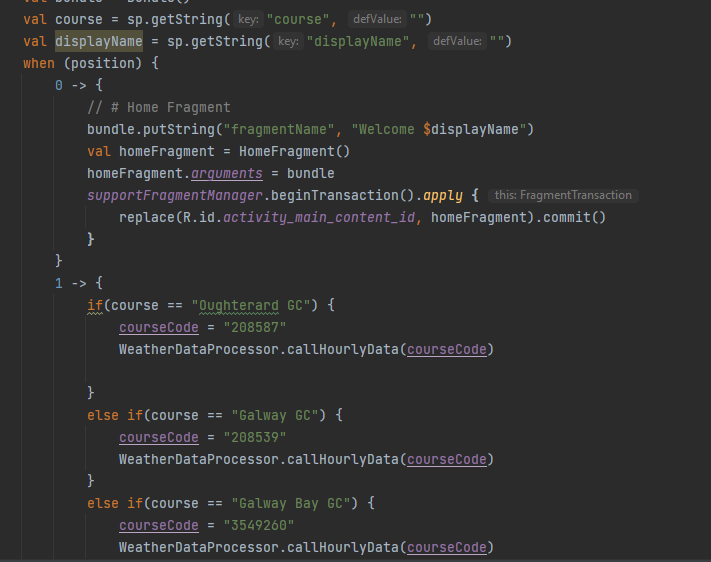
\includegraphics[width=12cm,height = 8cm]{img/CourseCodes.PNG}
    \caption{Course Codes used for API Request}
    \label{fig:altas config}
\end{figure}

\begin{figure}[H]
    \centering
    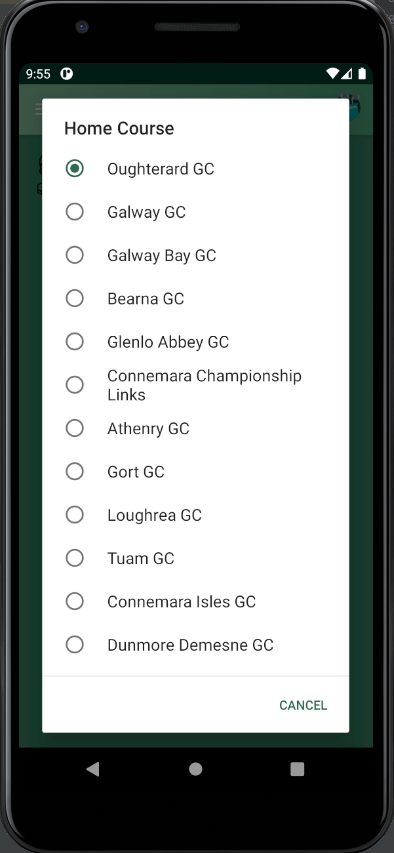
\includegraphics[width=7cm,height = 14cm]{img/InPhoneList.PNG}
    \caption{List of Courses used for Location}
    \label{fig:altas config}
\end{figure}
The above images show how based on the location the user has set as their chosen golf course, it will set the course code to that golf course and will then begin the first part in trying to retrieve the weather data for that particular golf course regardless of where the user is located.
\newline
Once the course has been selected, the course code is then passed to our callHourlyData Method which changes the course code for the API call the invokes the fetchCurrentJson method which then fetches the data.

\begin{figure}[H]
    \centering
    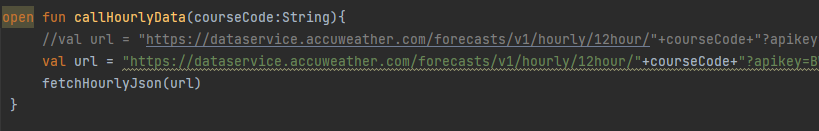
\includegraphics[width=16cm,height = 3cm]{img/APICall.PNG}
    \caption{Course Codes used for API Request}
    \label{fig:altas config}
\end{figure}
After the course code has been set, the data is then fetched using okhttp to fetch the JSON data from the API, while being fetched, the data is also stored locally using GSON in order to output the data to the user.
\newline
\newline
This data is stored in a Kotlin data class files in order for the specific data required for the hourly or current hour ratings to be created. By doing this it allows us to call each data type independently from the other data types so that we only use what we need to use.

\begin{figure}[H]
    \centering
    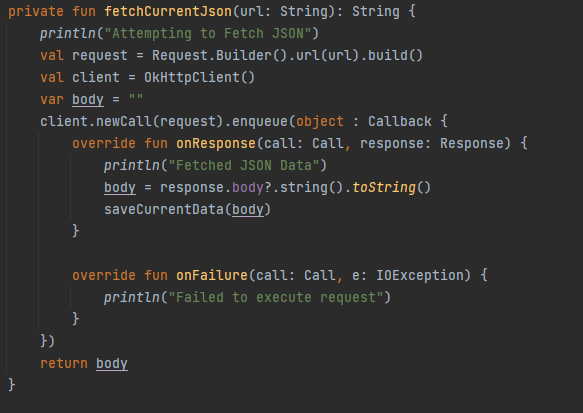
\includegraphics[width=12cm,height = 8cm]{img/DataFetch.PNG}
    \caption{Fetching of JSON Data using OKHTTP}
    \label{fig:altas config}
\end{figure}

\begin{figure}[H]
    \centering
    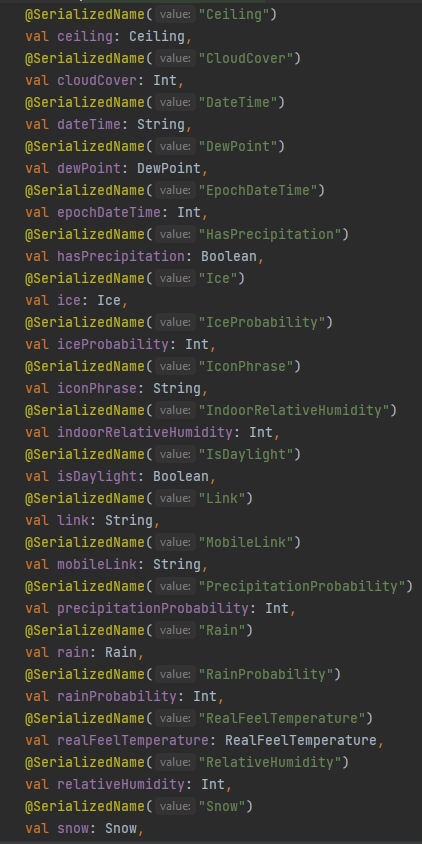
\includegraphics[width=10cm,height = 18cm]{img/DataExample.PNG}
    \caption{Example of the Data set used to store weather values}
    \label{fig:altas config}
\end{figure}

While saving the data locally this is where the function for calculating the is called and converted to a list along with all the data values being displayed to the user(Rainfall, WindSpeed, Temperature, Feels Like Temperature, Humidity, Hourly Rating).

\begin{figure}[H]
    \centering
    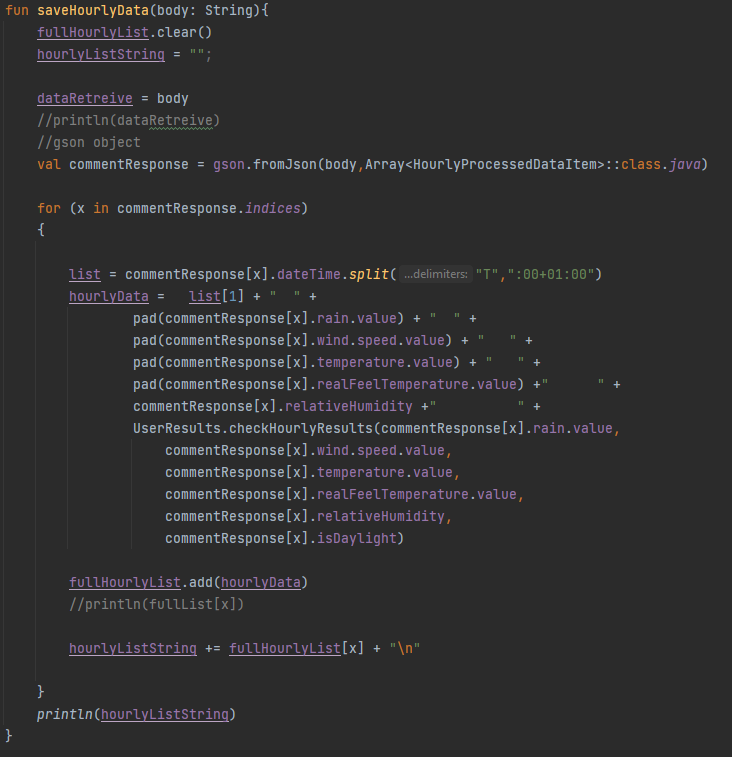
\includegraphics[width=12cm,height = 8cm]{img/DataStore.PNG}
    \caption{Storing of JSON data to Dataset Files}
    \label{fig:altas config}
\end{figure}

The function takes in the above values except for Hourly Rating and a value for if it is daytime and then compares them to a set of predetermined values for each of the five values and then each one is given a rating between 0 and 1 which then will give a rating between 0.0 and 5.0 or if it the hour is in night hours a rating of 0.0.

\begin{figure}[H]
    \centering
    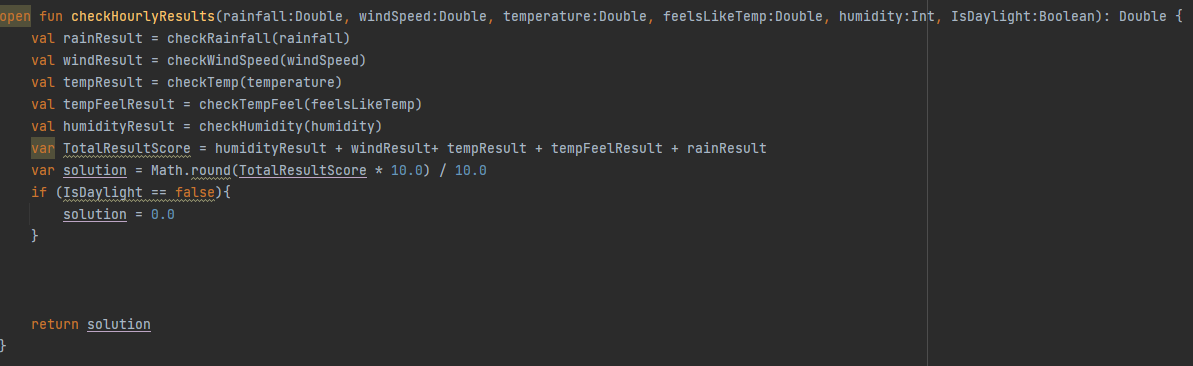
\includegraphics[width=16cm,height = 6cm]{img/DataComparison.PNG}
    \caption{Calculation of the rating}
    \label{fig:altas config}
\end{figure}

\begin{figure}[H]
    \centering
    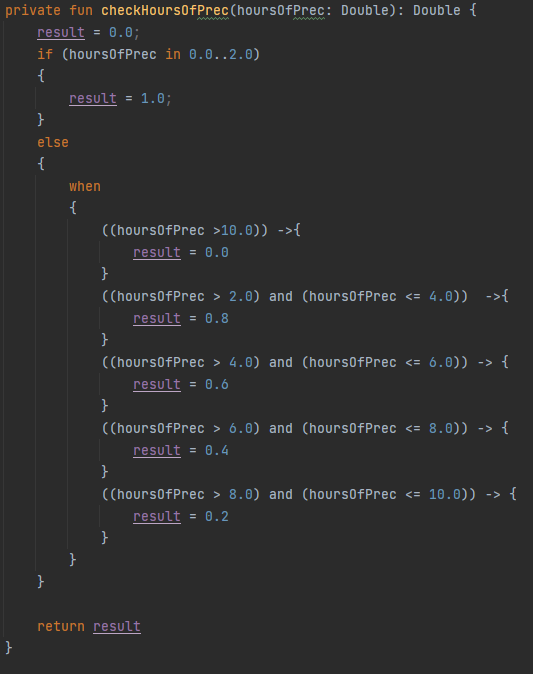
\includegraphics[width=10cm,height = 12cm]{img/DataComparisonExample.PNG}
    \caption{Example of how the data is compared}
    \label{fig:altas config}
\end{figure}

After all the data is processed it is then outputted to the user so that they can see the ratings for the next twelve hours or the current hour.

\begin{figure}[H]
    \centering
    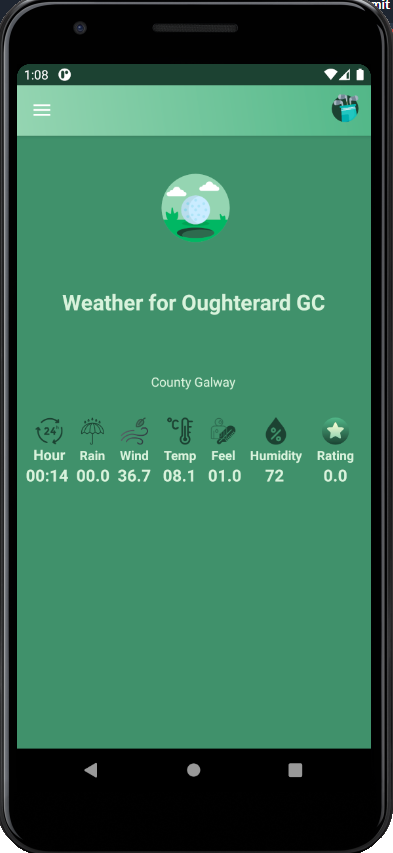
\includegraphics[width=7cm,height = 14cm]{img/CurrentDataOutput.PNG}
    \caption{Current Hour Weather Data}
    \label{fig:altas config}
\end{figure}

\begin{figure}[H]
    \centering
    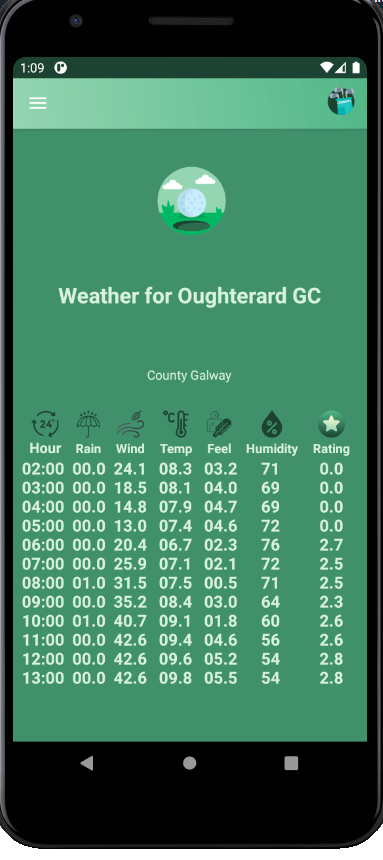
\includegraphics[width=7cm,height = 14cm]{img/HourlyDataOutput.PNG}
    \caption{ Next 12 Hours Weather Data}
    \label{fig:altas config}
\end{figure}


\chapter{System Evaluation}
In this chapter, we focused on the Testing, Evaluation, and Limitations of our Project. Our focus was to test how robust or project is by following by following the Agile methodology of Software Testing. We designed a Gantt Chart to outline sprints that break down the project into smaller parts which in turn, would be vigorously tested. The full Gantt chart can be viewed on the link below in our Github Repository.
\newline

\url{https://github.com/stevenJoyce/4thYearGroupProject/tree/main/TestingGuides}

\begin{figure}[H]
    \centering
    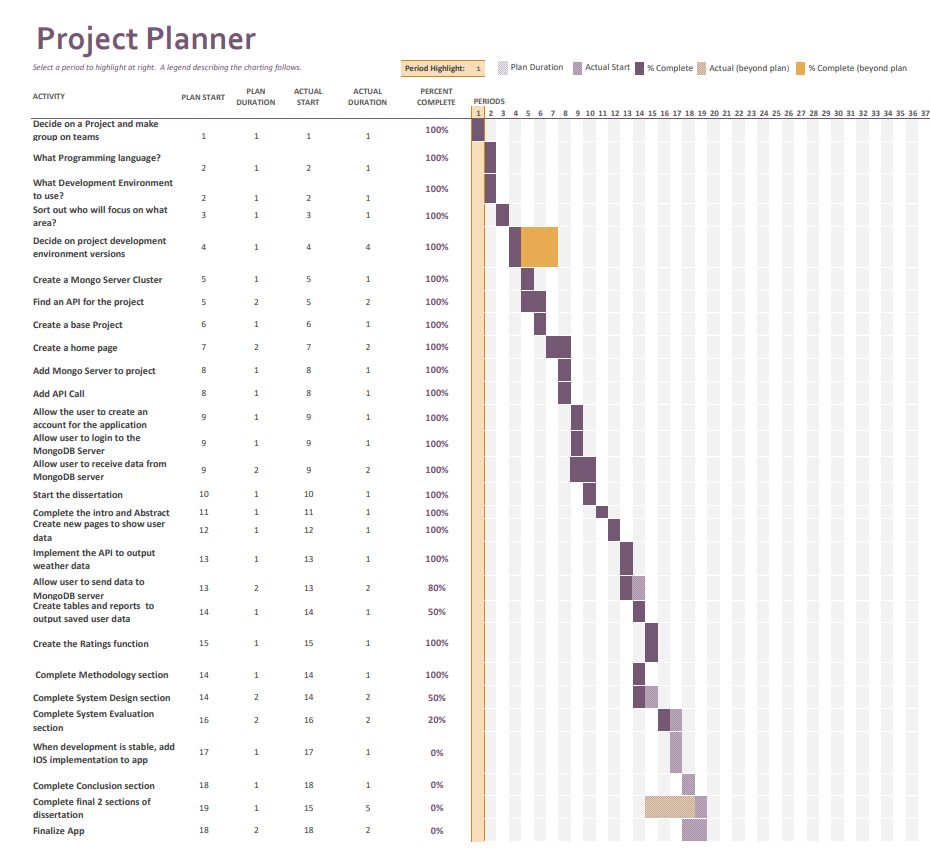
\includegraphics[width=15cm, height = 18cm]{img/Gantt.PNG}
    \caption{Test Case for successful Login}
    \label{fig:altas config}
\end{figure}

\section{Unit Testing}
For our project we have uses the Agile methodology to layout our plan. With this, testing is a major aspect of this methodology and as such, we created Test cases for each sprint and assigned a role for each team member. The roles assigned were as followed, Steven Joyce would create the unit tests which would be reviewed by Robert Donnelly before being implemented by Evan Greaney. These roles remained unchanged throughout the testing process.
\newline
\newline
The illustration below is an example of a test case used for running a successful login attempt. As seen below each case has an ID that is linked to the Gantt chart. The case uses the test data provided and requires prerequisites to be met for the test to be attempted. The test must follow the steps in a linear order for the case to be successful.
\begin{figure}[H]
    \centering
    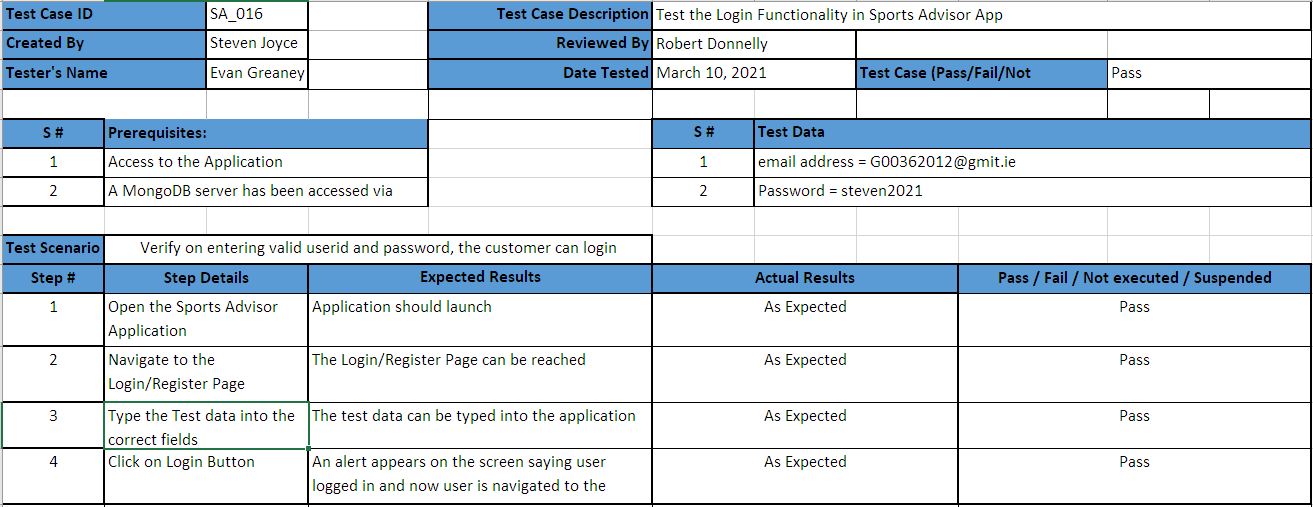
\includegraphics[width=15cm, height = 7.5cm]{img/TestCasePass.PNG}
    \caption{Test Case for successful Login}
    \label{fig:altas config}
\end{figure}
Some test cases are designed to confirm an unsuccessful outcome from a user's perspective. This can be seen in the image below, this test case although it passed most steps it failed to alert the user as to why they unsuccessfully logged in as the alert did not appear and ultimately the case failed. This case allowed us to implement alerts to summon at the correct time and place.
\begin{figure}[H]
    \centering
    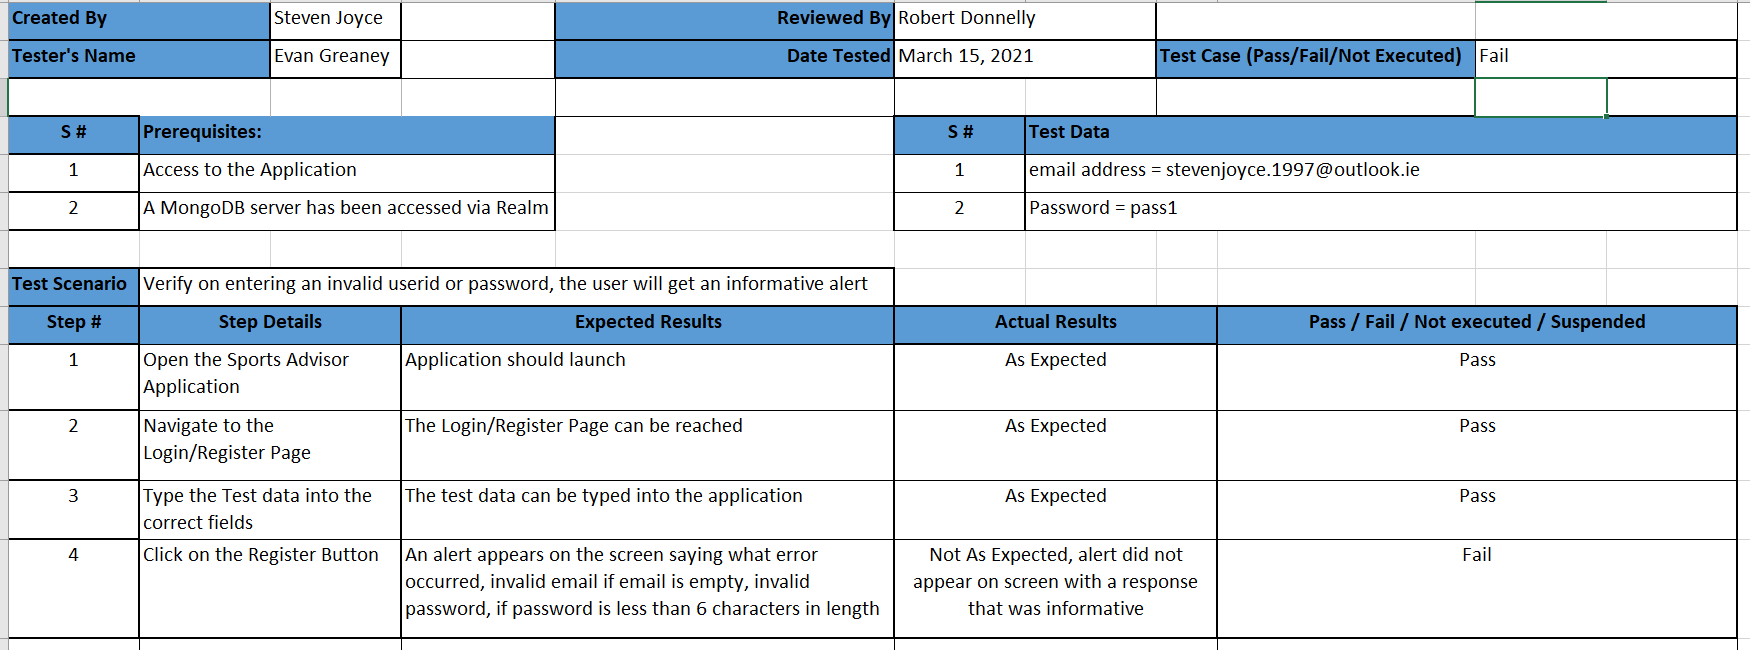
\includegraphics[width=15cm, height = 6.5cm]{img/TestCaseFail.PNG}
    \caption{Test Case for unsuccessful Login}
    \label{fig:altas config}
\end{figure}
With an understanding of what went wrong in the above test case, we implemented changes to our code that would give the user an informative alert that helps understand what error occurred. The screenshot below is a test case for the modified code with a successful outcome.
\begin{figure}[H]
    \centering
    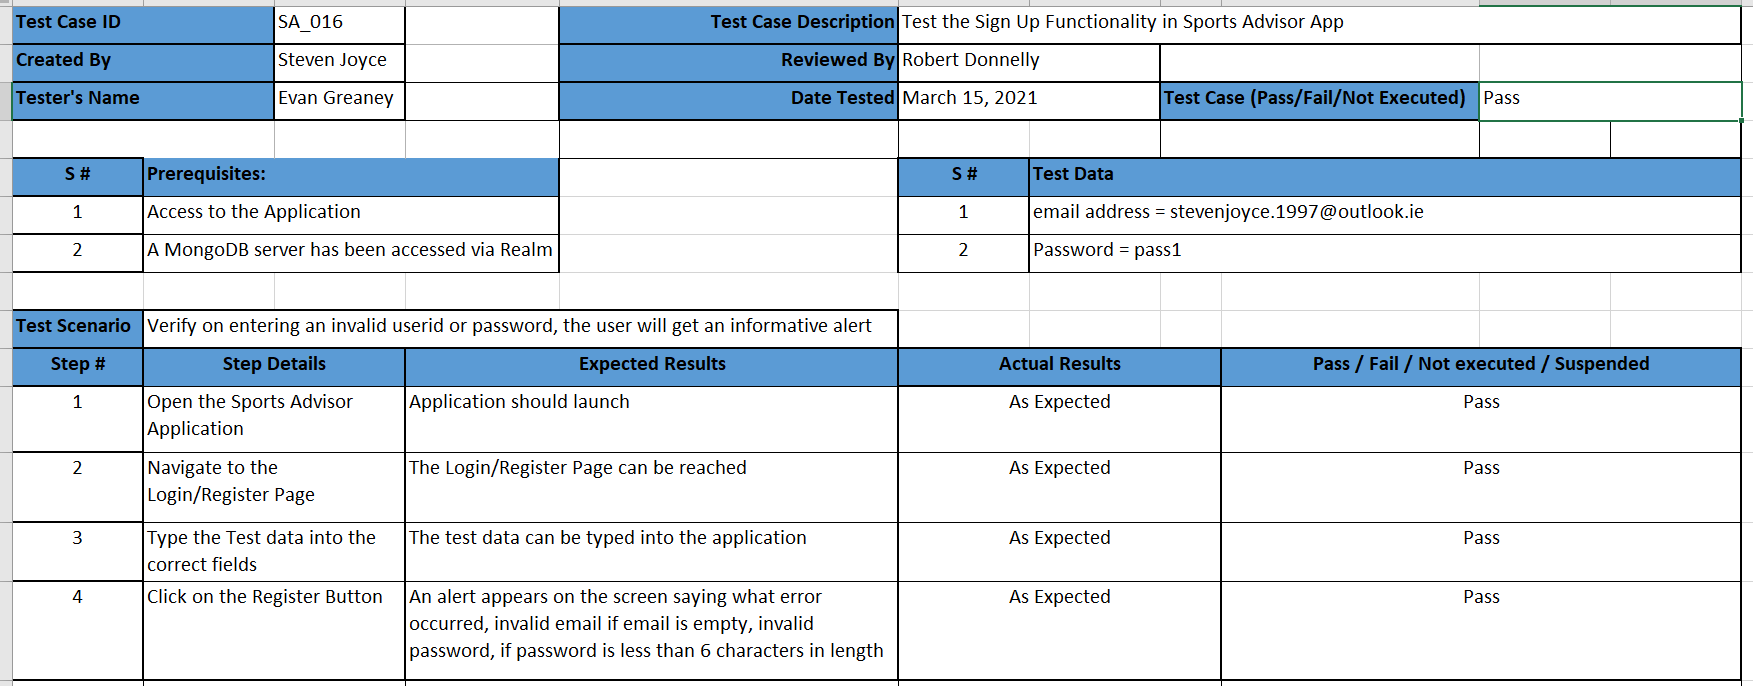
\includegraphics[width=15cm, height = 6.5 cm]{img/testCaseSignInError.PNG}
    \caption{Test Case for unsuccessful Login with Alerts}
    \label{fig:altas config}
\end{figure}
We did this type of testing for every feature of our application. This allowed us to debug our application regularly and efficiently. To see all of our test cases go to:  \url{https://github.com/stevenJoyce/4thYearGroupProject/tree/main/TestingGuides}
\section{Objectives Overview}
\subsubsection{Find a new programming language to learn independently}
The group's goal of learning a new programming language was achieved as the team gained skills and knowledge of Kotlin JVM, which the team members have no prior experience with this development tool before the past college year.
\subsubsection {Find a Methodology to best implement our idea}
Upon starting the year the team had chosen two main methodologies to consider, being Agile and Waterfall. Due to Agile being a better fit for an application, the team decided to pick this methodology as our preferred approach.
\subsubsection {Implement the methodology to create a project plan}
With our methodology choice, the way we approached our project plan was to split up the work into manageable parts, these were our sprints. The sprints were then handed out to each member of the team to complete within a given deadline of a set amount of weeks. The team had successfully created a plan. At the end of the planning process, a Gannt chart was created to be used to assign sprints to each member and manage the progress of the application's development.
\subsubsection {Find an architecture structure suitable to use}
With Kotlin being our language of choice, upon researching, the team discovered that it was mainly utilised for Android Development and that JetBrains, the company that is developing Kotlin also develops the IntelliJ IDE which supports the Android Studio SDK for android development. With this in mind, the team quickly and successfully came to an agreement that the application should be made in the JetBrains toolkit environment of IntelliJ and Android Studio.
\subsubsection {Utilize an environment for stable version control}
With our history of using GitHub it was a simple choice for the team to pick it as most developers struggle with learning a new version control environment so the team decided to stick with what they already had prior experience with. With the project on GitHub we were able to set up an interactive Issue board. This allowed issues to be assigned to individual team members and for the issue's progress to be tracked. It allowed each group member to access the latest version of the application from any machine which allowed for remote working, this was a vital aid for our team in a covid affected work environment.
\subsubsection {Establish a well structured base for the project}
To design and implement our Android application we needed a great IDE. Through our GitHub Student Developer Pack, we were given a free license for IntelliJ Ultimate. With our IDE we could create an emulator to test our application and call our MongoDB database to view any requests the application makes in real-time.
\subsubsection {Create a high quality front-end}
With Android Studio ADK being built into IntelliJ, we could design the page and write the code at the same time which helped us understand what we were trying to achieve for the end-user. We used a consistent colour scheme throughout the application XML layouts and drawable assets which resulted in a professional and appealing look and feel. We altered XML icons which would have not suited the application's look but through applying the colour scheme we made them match our application's theme. Every aspect from the drawer layout to buttons in one way or another conforms to the colour scheme of the application which in turn resulted in a high-quality front-end design.
\subsubsection {Find and deploy an API which our app can utilize}
After multiple attempts at using different APIs for our application, we decided on using the Accuweather API service. This allowed us to generate current weather conditions and the next 12 hours for the chosen area in Galway.
\subsubsection {Create a server service for the Application.}
With our prior knowledge and experience with MongoDB, it was a simple choice to make. We decided on using 2 aspects of MongoDB which are Atlas and Realm.
\subsubsection {Allow for user data to be protected and appropriately stored}
MongoDB Realm created a buffer between the server and application to filter unauthorized access to the user’s data. This a hidden layer of protection that filtered out any issues or unwarranted data.
\subsubsection {Use of a Location service to find user's desired location}
This objective was modified due to the API service, where the location can only be found using their custom location codes that a normal user would not have prior knowledge of. We changed into a list of all golf courses in Galway and allowed the user to choose a preferred golf course.
\subsubsection {Implement a login service which allows user to access their \newline protected data}
To view any user data, they have to sign to the application on the login page before setting their userID in the settings page. When the user goes to load its history they only view their own data.
\subsubsection {Design the Apps software to successfully implement the apps intended functionality}
The features that we originally set out to have on our application have all been achieved but the end result did not generate the original design plan we had intended due to limitations and a better understanding of what we wanted to achieve.
\subsubsection {Deploy our methodologies style of testing to ensure quality standards are met}
With the methodology testing approach we used, it favoured constant testing throughout the development cycle and as such allowed the team to fix unforeseen bugs and errors in our design and implementation as they happen. As developers, we tested our work after every change to the application with the built-in emulator. This ensured that we never committed non-functioning code to our repository.
\newpage
\section{Issues, limitations}
This section mainly pertains to the Issues and Limitations experienced by the team throughout the whole development lifecycle of the Application. Due to the nature of our project development tools and language being relatively new to ourselves and the wider coding community, there have been many challenges we have faced to develop this application that has needed to be resolved.
\subsection{IntelliJ}
\subsubsection{Limitations}
Our IDE only caused one limitation in the last stages of our development lifecycle when the IDE updated the Kotlin Language version, it forced updated our own project without consent and caused issues throughout all our .kt classes which led them to not be able to be rendered by the Gradle.
\newline
\newline
This resulted in us losing about 3 hours of development time due to us not realising what the root cause of the issue was. To fix this we had to look at our commit history through GitHub desktop to see what was changed file by file until we found the issue.
\newline
\newline
To resolve this we had to revert to a previous Kotlin language version of our project within the Project.xml file which then fixed our issue. This is a major limitation as it was outside of our control and we cannot be sure that this issue will not occur again and cause a loss in development time.

\begin{figure}[H]
    \centering
    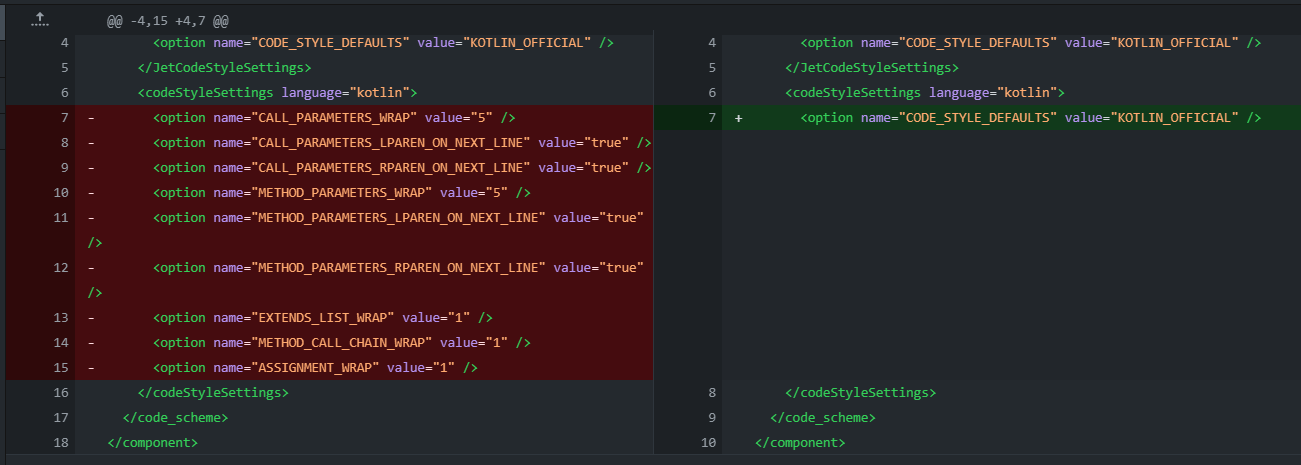
\includegraphics[width=16cm, height = 7.5cm]{img/Unplannedupdate.png}
    \caption{Unplanned update found in "Project.xml"}
    \label{fig:altas config}
\end{figure}

\subsection{Kotlin}
\subsubsection{Limitations}
The Kotlin language is not a difficult language to write code in but the lack of references to solutions outside of the main documentation was a hindrance to our project development. The code itself has been written in a way that is user friendly, with Java code being able to be converted in Kotlin instantly but if you want to look for code that is unconventional and outside of the norm for a class in either Java or Kotlin, you will most likely struggle to find any source to put you on the right path. The best you can hope for in a Java variation of the same code and convert it before modifying it to suit what you need,
This type of limitation will be rendered a non-issue in the future, as the language becomes more popular. 
\subsection{Android}
\subsubsection{Issues}
\subsubsection{Limitations}
\subsection{API Calling}
API calling was a major feature of our Application throughout our project as it allowed us to generate ratings for each hour shown and give a recommendation on which day to best play on but throughout our implementation of this feature we came across many limitations and issues within different parts of the project from the data retrieved to the API calls themselves and even limitations with pricing. Below will focus on the many issues and limitations that we came across when trying to implement this feature.

\subsubsection{Issues}
One of the first Issues we had before using the Accuweather API was when we were experimenting with multiple weather APIs, the first of which was the Met Eireann API. This was a fantastic API that would've given us all the data we needed and because it was designed for the island of Ireland, it would've been extremely accurate for the given locations but the issue with this API was its data it returned.
\newline
\newline
The data it returned was in XML format not JSON format and the technology that we were using to fetch and store the data required JSON data. We initially attempted to try to convert this data from XML to JSON but since we weren't storing this data to a file locally it wasn't possible to convert it to JSON. As a result, we had to search for another API to use.
\newline
\newline
The next major issue when trying to find an API to use for our project was when we tried to use an API called Openweather API, it had ticked nearly all the boxes for us, it was capable of finding the correct locations, retrieved back data in JSON format but unfortunately, when attempting to store the data it wasn’t able to be correctly stored in our data files as it came back as a set of JSON objects, not JSON data which would allow the data to be temporarily stored so that the data could be processed and return an output to a user. After testing these APIs we eventually came across the AccuWeather API which allowed us to retrieve, store and process as we saw fit.

\subsubsection{Limitations}
As we were working with these APIs we came across many limitations of them that wouldn't be called issues but limited our design and focus of the application to try and incorporate them into our application.
\newline
\newline
When attempting to work with the Open Weather API, one of the limitations that we had was that we had to use a third party to try and retrieve the location that the user was searching for based on either longitude and latitude or searching by name, we originally planned it to be searched for by name but found that when searching by name, due to Ireland having unusual city, town and our case golf course names, it was rather difficult to search via name for some golf courses and because of this, we had to remove the idea of allowing the user to search by name.
\newline
\newline
We then attempted to search by longitude and latitude where we attempted to get the longitude and latitude for the user using the Geolocation API by google but found that when we used it, it only returned back the users current location which hindered us from finding the locations of the golf courses we needed. Instead, we gave them a list of golf courses in Galway that when any one of them is clicked, it passes through the location code used by Accuweather to search for the course.
\newline
\newline
After trying many different APIs we eventually settled on the Accuweather API as it did just about everything we needed to complete the development with our project but came with just one limitation that was very similar to the issue found in the OpenWeather API was when we tried to fetch the five-day forecast, we could retrieve it with no issue but when trying to store it, our data could not handle JSON objects and instead threw errors, with this we had to redesign our what the user was able to see when generating the ratings and with that, we decided to check for the current conditions so that the user could accurately check the current conditions for their designated course as they got closer to the golf course.
\newline
\newline
The biggest limitation we had throughout all the APIs we used including the Accuweather API we settled upon was the limitation around pricing. As we are students we could not afford to purchase API packages to get more API requests per month and to have more API fetch types like searching for the weather for the next 72 hours instead of 12 hours and because of this, we had to design the app to be checked the day you plan to play golf to check for the best hours to play instead of being able to plan a couple of days ahead.
\newline
\newline
This also hindered our development as we could only make 50 API fetch re- quests a day and found when trying to test this functionality after only an hour and a half into development we were unable to continue testing until the following day.
\subsection{MongoDB}
With the way, we used MongoDB with our application we needed to have a MongoDB Realm Application. Realm was only brought by MongoDB realm in April 2019 for \$39 million. The integrated system was only released for General Use on February 4th, 2021. We had been using this system since October 2020. We were allowed access to this due to already having a MongoDB account and can be seen as an experienced MongoDB NoSQL Database User.
\subsubsection{Issues}
One of the lingering issues we had with connecting to MongoDB from a Kotlin Android Application was that MongoDB 4.4 has been in beta since June 2020. This is the only version of MongoDB that can use with MongoDB Realm Sync. This issue has led to some aspects of MongoDB not being documented fully and integration of Kotlin language with query searches being limited. We wanted to only output 5 of the 7 fields we had stored in our MongoDB Database but due to the integration of Kotlin code now being finished, we could only remove 1 of the fields. We hope that in the future this issue can be resolved and our application can be modified to allow the user to choose what fields it wants to generate their data from.
\subsubsection{Limitations}
With our application, we have a way for the user to create an account to store data within the MongoDB database. At this moment we do not have a way to link a userID to a specific email/password for better user data protection. This would also render the settings userID as redundant because we could set that value when we log in to the application. This would make all collections that have that value to only open when the email and password that is linked to it is inputted into the application and sent to the MongoDB realm app to valid login credentials.
\newline
When a user registers an email, due to us not owning a domain that can be used to send an email address verification link, the email address at this time does not get verified. The only real safeguard is when to try to register the same email again, you will be given an alert that states \"email already has an account\". This can be very annoying for a user because if you register with an email address that is spelt incorrectly, you will not be told with an alert. The email will automatically be verified by the MongoDB database. The sign-in function with MongoDB Sync was riddled with bugs and is unusable. This led us to remove it from the application entirely until it is fixed. \newline We hope that when the Realm Sync is fully functioning that this aspect of the system is working fully and we can use either the function call or purchase a domain for email verification.
\subsection{Overleaf}
For writing our dissertation, we decided to use Overleaf due to our knowledge of overleaf from a previous module. The biggest issue we found with overleaf was that you could not have more than 2 people with access to the same project. This led to issues with making sure the dissertation that every member of the group had accessed to was the latest version. The only solution to this, would be to subscribe to Overleaf with a monthly fee that every member of the group would have to pay.  
\newline
\newline
\section {Issues Overcame}
\subsection{IntelliJ}
With the base version of IntelliJ we could not access a MongoDB database to view the collection data or any changes we had made in the project without leaving IntelliJ and signing in to our MongoDB Project and go to Atlas to view the database collections. This was a big issue with our IDE, as we needed to view all changes instantly so we could find any bugs straight away and patch the problem. \newline
The way we overcame this, was to upgrade our IDE to IntelliJ Ultimate. This allowed the database tool inside Net Brains to be used in conjunction with IntelliJ. The database tool allows us to sign into our MongoDB database inside of IntelliJ and view all the collections in our database. We could also see any changes made to the database with a refresh of the tool. This helped us see what was happening quickly and be able to understand what the issue was and how to fix it.
\newpage
\subsection{MongoDB}
\subsubsection{MongoDB Atlas Cluster Integration}
The original MongoDB Atlas Cluster region we have designated for our application was not able to run MongoDB 4.4. The use of MongoDB 4.4 was essential to our app because it allowed MongoDB Realm integration. We first had our cluster region set as AWS / Ireland (eu-west-1). This cluster still uses MongoDB 4.2 and could not be used for our application. We had to rebuild our MongoDB Atlas Cluster set up and change the region to AWS N. Virginia (us-east-1). This was the closest region to Ireland that was still a part of the the free tier and was integrated with MongoDB 4.4.

\subsubsection{Connecting the Android App to MongoDB}
One of the major issues we had with the project was getting access to the Database while the application was running, this led us to find MongoDB Realm. this is a new software to the MongoDB Services. It has been slowly integrated into the MongoDB database since the start of 2020, the general public has only been able to use this since February. The software created an app on the server side to be used as a gateway between an application and a MongoDB database, The use of the this software rapidly changed how we could utilize a database with our application, With only a few lines of code, we could connect to the app to the database and we easy to understand. The documentation to use it with Kaitlin is not finished yet but we could resolve any issues ourselves.
\subsubsection{MongoDB returning collections}
With MongoDB not enabling a userID to be linked to a specific email and password, we had to find a way to protect user data while printing out data the user has stored in the application. To solve this issue, we created a userID field in the settings. The user will create a unique identifier in this location that can be used throughout the app. When the user saves a score in the score fragment, the userID is sent along with all the other values. When we enter the User History page of the Android Application, the onCreate function will run a search of the database and bring back every collection associated with the userID that the user has defined on the settings page.

\subsubsection{MongoDB adding Collections}
The MongoDB Documentation does not give you the Kotlin code equivalent to adding a collection that is populated with both user input and generated input. To overcome this we had to send all the user inputs to a function before that function saves the variables into a local variable to be used inside the function itself. The data is then sent to the collection with the insertOne method found in the ScoreFragment.kt file. It used .append for every field to add a new value in the specified field.
\section{Future of Application}
\subsection{Multi-platform Application}
In our future development plans for our application is to introduce our app to more platforms, we originally planned for our app to be deployed to both android and iOS from the beginning but to focus on android to allow for a more robust application to be designed.
\subsubsection{iOS}
We hoped to include iOS as part of our plan for development of our application from the beginning but due to iOS being in alpha stability for Kotlin App development\cite{ref2} we had to remove it from our plan due to its unreliability and hold off until the component becomes more reliable so that we can implement it when its status improves.
\subsubsection{Harmony OS}
When Harmony OS becomes more prevalent on the wider market, we plan to redisgn our app to build a version of our app to be deployed to Harmony OS. At the moment Harmony OS only supports Java, C and JavaScript with plans for kotlin to be supported to later in its development life cycle. When this is implemented and supported, we will then work to add our App to this platform.
\newline
\subsection{MongoDB Realm}
\subsubsection{Integration}
With MongoDB Realm still not fully finished yet, we will see major features added for use with Kotlin. This includes running multiple queries and being able to get back the data in a string, not a document. These 2 features alone will change the way we get back collections from the database. We would be able to only bring back data that the user wants to see rather than everything except from the ObjectID. 
\newline
When the login function is fully functional we will be able to verify email addresses and be able to link a UserID to a specific User. This will improve the security of user data immensely. The email verification would help users who may make a mistake in the email input and may not know what they did wrong.
\newline
In the future we would like to be able to link accounts to either your Facebook or WhatsApp to allow the user to share their golf scores with their friends.
\newline
MongoDB allows users to sign up with a Facebook, Google or Apple account. This feature is another that we would like to add to the application to allow the user to sign up in a way that is less time consuming and will not require email verification.
\subsection{API Call Licensing}
I
\subsubsection{Paid License}
Our
\subsection{Nationwide/Global}
\subsubsection{Ireland}
Irish
\subsubsection{Major Golf Courses}
US
\subsection{New Features}
\subsubsection{Wind Direction}
Arrow
\subsubsection{AI}
Hints
\begin{itemize}
\item Prove that your software is robust. How? Testing etc.
\item Use performance benchmarks (space and time) if algorithmic.
\item Measure the outcomes / outputs of your system / software against the objectives from the Introduction.
\item Highlight any limitations or opportunities in your approach or technologies used.
\end{itemize}
\chapter{Conclusion}
About three pages.
\begin{itemize}
\item Briefly summarise your context and objectives (a few lines).
\item Highlight your findings from the evaluation section / chapter and any opportunities identified.
\end{itemize}
\chapter{References}

\begin{thebibliography}{9}
\bibitem{ref1} {title={OkHttp},url={https://square.github.io/okhttp/}, journal={OkHttp}, author={Square, Inc.}}
\bibitem{ref2} {title={Stability of components},
url={https://kotlinlang.org/docs/components-stability.html}, journal={Kotlin}, author={IntelliJ}}

\end{thebibliography}
\chapter{Appendices}